\RequirePackage{silence}
\documentclass[10pt,aspectratio=1610,t,xcolor={dvipsnames}]{beamer}
\usepackage{etex}
\usepackage[dvipsnames]{xcolor}
\usepackage{color, colortbl}
\usetheme[
%%% options passed to the outer them
%    hidetitle,           % hide the (short) title in the sidebar
%    hideauthor,          % hide the (short) author in the sidebar
%    hideinstitute,       % hide the (short) institute in the bottom of the sidebar
%    shownavsym,          % show the navigation symbols
%    width=2cm,           % width of the sidebar (default is 2 cm)
%    hideothersubsections,% hide all subsections but the subsections in the current section
%    hideallsubsections,  % hide all subsections
    left               % right of left position of sidebar (default is right)
%%% options passed to the color theme
%    lightheaderbg,       % use a light header background
  ]{AAUsidebar}

% If you want to change the colors of the various elements in the theme, edit and uncomment the following lines
% Change the bar and sidebar colors:
%\setbeamercolor{AAUsidebar}{fg=red!20,bg=red}
%\setbeamercolor{sidebar}{bg=red!20}
% Change the color of the structural elements:
%\setbeamercolor{structure}{fg=red}
% Change the frame title text color:
%\setbeamercolor{frametitle}{fg=blue}
% Change the normal text color background:
%\setbeamercolor{normal text}{bg=gray!10}
% ... and you can of course change a lot more - see the beamer user manual.
\WarningsOff
%%%% WARNING HACKS %%%%
%\hfuzz=\maxdimen
\hbadness=\maxdimen
\vbadness=\maxdimen
%\vfuzz=\maxdimen

\usepackage{graphicx}
\usepackage{multimedia}
\usepackage{subcaption}
\captionsetup{compatibility=false}
%\setbeamercovered{transparent}

\usepackage[utf8]{inputenc}
\usepackage[english]{babel}
\usepackage[T1]{fontenc}
% Or whatever. Note that the encoding and the font should match. If T1
% does not look nice, try deleting the line with the fontenc.
\usepackage{helvet}




% colored hyperlinks
\newcommand{\chref}[2]{%
  \href{#1}{{\usebeamercolor[bg]{AAUsidebar}#2}}%
}

\title[Agenda]% optional, use only with long paper titles
{Optimal Control for Water Distribution}

%\subtitle{Total fizz}  % could also be a conference name

\date{June 26, 2017}

\author[Group 830] % optional, use only with lots of authors
{
	Group 830 \\
  \scalebox{0.6}{Daniel Bähner Andersen}\\ \vspace{-1mm}
  \scalebox{0.6}{Ignacio Trojaola Bolinaga}\\ \vspace{-1mm}
  \scalebox{0.6}{Krisztian Mark Balla}\\ \vspace{-1mm}
  \scalebox{0.6}{Nicolaj Vinkel Christensen}\\ \vspace{-1mm}
  \scalebox{0.6}{Simon Bjerre Krogh}\\ \vspace{-1mm}
  %%\href{mailto:XX13@student.aau.dk}{{\tt mksi13@student.aau.dk}}
}
% - Give the names in the same order as they appear in the paper.
% - Use the \inst{?} command only if the authors have different
%   affiliation. See the beamer manual for an example

\institute[
%  {\includegraphics[scale=0.2]{aau_segl}}\\ %insert a company, department or university logo
  Dept.\ of Electronic Systems\\
  Aalborg University\\
  Denmark
] % optional - is placed in the bottom of the sidebar on every slide
{% is placed on the title page
  Department of Electronic Systems\\
  Aalborg University\\
  Denmark
  
  %there must be an empty line above this line - otherwise some unwanted space is added between the university and the country (I do not know why;( )
}


% specify a logo on the titlepage (you can specify additional logos an include them in 
% institute command below
\pgfdeclareimage[height=1.5cm]{titlepagelogo}{AAUgraphics/aau_logo_new} % placed on the title page
%\pgfdeclareimage[height=1.5cm]{titlepagelogo2}{graphics/aau_logo_new} % placed on the title page
\titlegraphic{% is placed on the bottom of the title page
  \pgfuseimage{titlepagelogo}
%  \hspace{1cm}\pgfuseimage{titlepagelogo2}
}

%%%%%%%%%%%%%%%EXTRA FEATURES%%%%%%%%%%%%%%%
\usepackage{schemabloc}
\usetikzlibrary{circuits}
\usepackage{tikz}
\usetikzlibrary{shapes,arrows}
\usepackage{pgfplots}
\usetikzlibrary{plotmarks}
\pgfplotsset{compat=newest}
\pgfplotsset{filter discard warning=false}
\usepackage[americanresistors,americaninductors,american voltages]{circuitikz}
\usepackage{fancybox}
\usepackage[absolute,overlay]{textpos}
\usepackage{graphicx,import}

%%%%%%%%%%%%%%%TIKZ MAGIC%%%%%%%%%%%%%%%
\tikzstyle{block} = [draw, fill=blue!20, rectangle, minimum height=3em, minimum width=6em]
\tikzstyle{Integrator} = [draw, fill=blue!20, rectangle, minimum height=5mm, minimum width=5mm]
\tikzstyle{Twolineblock} = [draw, fill=blue!20, rectangle, minimum height=3em, minimum width=6em, text width = 6em, align=center]       
\tikzstyle{sum} = [draw, fill=blue!20, circle, node distance=1cm]
\tikzstyle{input} = [coordinate]
\tikzstyle{output} = [coordinate]
\tikzstyle{pinstyle} = [pin edge={to-,thin,black}]
\tikzstyle{box} = [draw,rounded corners, minimum height=15mm, minimum width=20mm, align=center, text centered]
\tikzstyle{BlackBox} = [draw, fill=black, rounded corners, minimum height=15mm, minimum width=20mm, align=center, text=white, text centered]
\tikzstyle{FlowIF} = [diamond, draw, fill=blue!20, text width=8.5em, text badly centered, node distance=3cm, inner sep=0pt,align=center,aspect=3]
\tikzstyle{FlowBlock} = [rectangle, draw, fill=blue!20, text width=8em, text centered, rounded corners, minimum height=3em]
\tikzstyle{FlowCloud} = [draw, ellipse,fill=red!20, node distance=3cm, minimum height=2em]
\tikzstyle{TestBox} = [rectangle,draw, fill=black!20, minimum height=8mm, minimum width=8mm]
\tikzstyle{TestDiamond} = [diamond, draw, fill=black!20, minimum height=10.5mm, minimum width=10.5mm]
\tikzstyle{TestBox} = [rectangle,draw, fill=black!20, minimum height=8mm, minimum width=8mm]
\tikzstyle{TestCircle} = [circle, draw, fill=black!20, minimum height=6mm, minimum width=6mm]
\tikzstyle{TestTable} = [rectangle, draw, fill=black!60, minimum height=0.01mm, minimum width=9mm, text=white]
\tikzstyle{TestBoxSmall} = [rectangle,draw, fill=black!, minimum height=8mm, minimum width=8mm,text=white]
\tikzstyle{LegendBox} = [rectangle,draw, minimum height=7mm, minimum width=20mm]
\tikzstyle{Sysbox} = [draw,rounded corners, minimum height=15mm, minimum width=9em, align=center, text centered,text width = 10.5em]
\tikzstyle{SysBlackBox} = [draw, fill=black, text=white, rounded corners, minimum height=15mm, minimum width=9em, align=center, text centered,text width = 10em]




\begin{document}
\usetikzlibrary{shapes,arrows}
\usetikzlibrary{plotmarks}
\pgfplotsset{compat=newest}
\pgfplotsset{filter discard warning=false}

\pgfdeclarelayer{bg}    % declare background layer
\pgfsetlayers{bg,main}


%\usepackage{silence}
%\WarningsOff[pgfplots]
%\WarningFilter{latex}{Marginpar on page}
%\WarningsOff[latex]


%%% Tikz Magic %%%
\tikzstyle{block} = [draw,rounded corners , rectangle, minimum height=3em, minimum width=6em]
\tikzstyle{Integrator} = [draw, fill=blue!20, rectangle, minimum height=5mm, minimum width=5mm]
\tikzstyle{Twolineblock} = [draw,rounded corners , rectangle, minimum height=3em, minimum width=6em, text width = 6em, align=center]     
\tikzstyle{sum} = [draw, fill=blue!20, circle, node distance=1cm]
\tikzstyle{input} = [coordinate]
\tikzstyle{output} = [coordinate]
\tikzstyle{pinstyle} = [pin edge={to-,thin,black}]
\tikzstyle{box} = [draw,rounded corners, minimum height=15mm, minimum width=20mm, align=center, text centered]
\tikzstyle{BlackBox} = [draw, fill=black, rounded corners, minimum height=15mm, minimum width=20mm, align=center, text=white, text centered]
\tikzstyle{FlowIF} = [diamond, draw, fill=blue!20, text width=8.5em, text badly centered, node distance=3cm, inner sep=0pt,align=center,aspect=3]
\tikzstyle{FlowBlock} = [rectangle, draw, fill=blue!20, text width=8em, text centered, rounded corners, minimum height=3em]
\tikzstyle{FlowCloud} = [draw, ellipse,fill=red!20, node distance=3cm, minimum height=2em]
\tikzstyle{TestBox} = [rectangle,draw, fill=black!20, minimum height=8mm, minimum width=8mm]
\tikzstyle{TestDiamond} = [diamond, draw, fill=black!20, minimum height=10.5mm, minimum width=10.5mm]
\tikzstyle{TestBox} = [rectangle,draw, fill=black!20, minimum height=8mm, minimum width=8mm]
\tikzstyle{TestCircle} = [circle, draw, fill=black!20, minimum height=6mm, minimum width=6mm]
\tikzstyle{TestTable} = [rectangle, draw, fill=black!60, minimum height=0.01mm, minimum width=9mm, text=white]
\tikzstyle{TestBoxSmall} = [rectangle,draw, fill=black!, minimum height=8mm, minimum width=8mm,text=white]
\tikzstyle{LegendBox} = [rectangle,draw, minimum height=7mm, minimum width=20mm]
\tikzstyle{Sysbox} = [draw,rounded corners, minimum height=15mm, minimum width=9em, align=center, text centered,text width = 10.5em]
\tikzstyle{SysBlackBox} = [draw, fill=black, text=white, rounded corners, minimum height=15mm, minimum width=9em, align=center, text centered,text width = 10em]
\tikzstyle{PreAmpBox} = [rectangle,draw, fill=black!20, minimum height=8mm, minimum width=12mm]
\tikzstyle{gain} = [fill=white, draw, rectangle, minimum height=2.5em, minimum width=2.5em]
\tikzstyle{summation} = [draw, minimum size=0.75cm, circle, node distance=1.75cm]












%% Its a pie chart!! %%%
\definecolor{rosso}{RGB}{220,57,18}
\definecolor{giallo}{RGB}{255,153,0}
\definecolor{blu}{RGB}{102,140,217}
\definecolor{verde}{RGB}{16,150,24}
\definecolor{viola}{RGB}{153,0,153}

\makeatletter

\tikzstyle{chart}=[
    legend label/.style={font={\scriptsize},anchor=west,align=left},
    legend box/.style={rectangle, draw, minimum size=5pt},
    axis/.style={black,semithick,->},
    axis label/.style={anchor=east,font={\tiny}},
]

\tikzstyle{bar chart}=[
    chart,
    bar width/.code={
        \pgfmathparse{##1/2}
        \global\let\bar@w\pgfmathresult
    },
    bar/.style={very thick, draw=white},
    bar label/.style={font={\bf\small},anchor=north},
    bar value/.style={font={\footnotesize}},
    bar width=.75,
]

\tikzstyle{pie chart}=[
    chart,
    slice/.style={line cap=round, line join=round, very thick,draw=white},
    pie title/.style={font={\bf}},
    slice type/.style 2 args={
        ##1/.style={fill=##2},
        values of ##1/.style={}
    }
]

\pgfdeclarelayer{background}
\pgfdeclarelayer{foreground}
\pgfsetlayers{background,main,foreground}



\newcommand{\pie}[3][]{
    \begin{scope}[#1]
    \pgfmathsetmacro{\curA}{90}
    \pgfmathsetmacro{\r}{1}
    \def\c{(0,0)}
    \node[pie title] at (90:1.3) {#2};
    \foreach \v/\s in{#3}{
        \pgfmathsetmacro{\deltaA}{\v/100*360}
        \pgfmathsetmacro{\nextA}{\curA + \deltaA}
        \pgfmathsetmacro{\midA}{(\curA+\nextA)/2}

        \path[slice,\s] \c
            -- +(\curA:\r)
            arc (\curA:\nextA:\r)
            -- cycle;
        \pgfmathsetmacro{\d}{max((\deltaA * -(.5/50) + 1) , .5)}

        \begin{pgfonlayer}{foreground}
        \path \c -- node[pos=\d,pie values,values of \s]{$\v\%$} +(\midA:\r);
        \end{pgfonlayer}

        \global\let\curA\nextA
    }
    \end{scope}
}




%% Cutom legned entry
\newenvironment{customlegend}[1][]{%
	\begingroup
	% inits/clears the lists (which might be populated from previous
	% axes):
	\csname pgfplots@init@cleared@structures\endcsname
	\pgfplotsset{#1}%
}{%
% draws the legend:
\csname pgfplots@createlegend\endcsname
\endgroup
}%

% makes \addlegendimage available (typically only available within an
% axis environment):
\def\addlegendimage{\csname pgfplots@addlegendimage\endcsname}

\usetikzlibrary{arrows}
\tikzset{>=stealth}


%% Its Color time:
\definecolor{MATLABblue}{rgb}{0,0.4470,0.7410}
\definecolor{MATLABorange}{rgb}{0.85,0.3250,0.0980}
\definecolor{MATLAByellow}{rgb}{0.929,0.6940,0.1250}
\definecolor{MATLABpurple}{rgb}{0.494,0.1840,0.5560}
\definecolor{MATLABgreen}{rgb}{0.466,0.6740,0.1880}
\definecolor{MATLABbabyblue}{rgb}{0.301,0.7450,0.9330}
\definecolor{MATLABred}{rgb}{0.635,0.0780,0.1840}
%% Loopback color
\definecolor{MATLABblack}{rgb}{0,0,0}

%% Microphone Colors
\definecolor{M1}{rgb}{0,0.4470,0.7410}
\definecolor{M2}{rgb}{0.85,0.3250,0.0980}
\definecolor{M3}{rgb}{0.929,0.6940,0.1250}
\definecolor{M4}{rgb}{0.494,0.1840,0.5560}
\definecolor{M5}{rgb}{0.466,0.6740,0.1880}
\definecolor{M6}{rgb}{0.301,0.7450,0.9330}
\definecolor{M7}{rgb}{0.635,0.0780,0.1840}
\definecolor{M8}{rgb}{0,0,1}
\definecolor{M9}{rgb}{0,0.5,1}
\definecolor{M10}{rgb}{0,1,0.5}
\definecolor{M11}{rgb}{0,1,1}
\definecolor{M12}{rgb}{0.5,1,0.5}
\definecolor{M13}{rgb}{1,0.5,0}
\definecolor{M14}{rgb}{1,0,0}
\definecolor{M15}{rgb}{0.5,0,0}

\newcommand*\circled[1]{\tikz[baseline=(char.base)]{
		\node[shape=circle,draw,inner sep=2pt] (char) {#1};}}



\newenvironment{sbmatrix}[1]
{\def\mysubscript{#1}\mathop\bgroup\begin{bmatrix}}
	{\end{bmatrix}\egroup_{\textstyle\mathstrut\mysubscript}}

\usetikzlibrary{matrix,calc}
\tikzstyle{loosely dotted}=[dash pattern=on 2\pgflinewidth off 24pt]

% \makeatletter
% \renewcommand{\todo}[2][]{\tikzexternaldisable\@todo[#1]{#2}\tikzexternalenable}
% \makeatother

% %\makeatletter
% %\renewcommand{\missingfigure}[2][]{\tikzexternaldisable\@missingfigure[#1]{#2}\tikzexternalenable}
% %\makeatother

% \let\oldmissingfigure\missingfigure
% \renewcommand{\missingfigure}[2][]{\tikzexternaldisable\oldmissingfigure[#1]{#2}\tikzexternalenable}
% the titlepage
{\aauwavesbg%
\begin{frame}[plain,noframenumbering] % the plain option removes the sidebar and header from the title page
  \titlepage
\end{frame}}
%%%%%%%%%%%%%%%%

% TOC
\begin{frame}{Agenda}{}
\tableofcontents
\end{frame}



%%%%%%%%%%%%%%%%
\section{Introduction}
%%%%%%%%%%%% MID WAY AGENDA %%%%%%%%%%%%%%
%\begin{frame}<beamer>
%\frametitle{Daniel Bähner Andersen}
%\tableofcontents[currentsection]
%\end{frame}
%%%%%%%%%%%% MID WAY AGENDA %%%%%%%%%%%%%%

\begin{frame}{Introduction}{}
    \begin{itemize}            
	\item<1-> Water distribution network
	    \begin{itemize}  
			\item<1-> Necessary infrastructure 
			\item<1-> High energy consumption 
		\end{itemize}   
\end{itemize}
\begin{itemize}	
	\item<2-> Possible solution 
	\begin{itemize}	
		\item<2-> Introduction of water tower
		\item<2-> Advance control that ensure satisfying performance
	\end{itemize}
\end{itemize}
\begin{itemize}	
		\item<3-> \textit{How can a water tower be implemented in a water distribution network and controlled to minimize the cost of running the distribution network without violating constraints and compromising the water quality.}
    \end{itemize}           
\end{frame}



\begin{frame}{System description}{System description}
\begin{figure}[H]
\centering
%\tikzsetnextfilename{sys_model_overview}
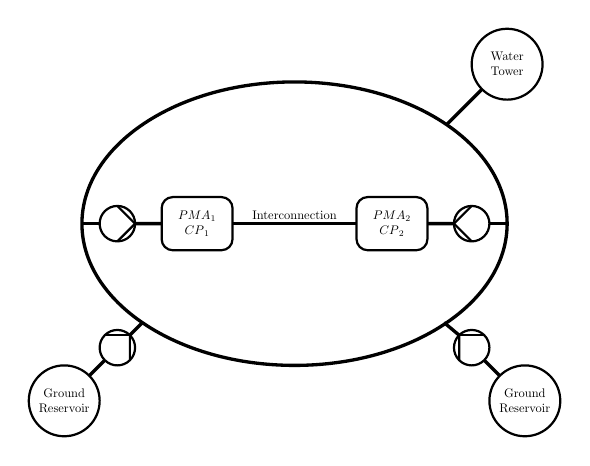
\begin{tikzpicture}[scale=0.45,transform shape]
\tikzstyle{box} = [draw,thick,rounded corners, minimum height=15mm, minimum width=20mm, align=center, text centered]
%Main Ring
\draw[very thick] (7,5.5) ellipse (6 and 4);
%Pump
\draw[thick,transform shape] (2,5.5) circle (0.5);
\draw[thick,transform shape] (2.5,5.5) -- (2,6);
\draw[thick,transform shape] (2.5,5.5) -- (2,5);
%Pump
\begin{scope} [rotate around={180:(12,5.5)}]
\draw[thick,transform shape] (12,5.5) circle (0.5);
\draw[thick,transform shape] (12.5,5.5) -- (12,6);
\draw[thick,transform shape] (12.5,5.5) -- (12,5);
\end{scope}
%Pump
\begin{scope} [rotate around={135:(12,2)}]
\draw[thick,transform shape] (12,2) circle (0.5);
\draw[thick,transform shape] (12.5,2) -- (12,2.5);
\draw[thick,transform shape] (12.5,2) -- (12,1.5);
\end{scope}
%Pump
\begin{scope} [rotate around={45:(2,2)}]
\draw[thick,transform shape] (2,2) circle (0.5);
\draw[thick,transform shape] (2.5,2) -- (2,2.5);
\draw[thick,transform shape] (2.5,2) -- (2,1.5);
\end{scope}
%Reservoirs
\node[thick,draw,circle,minimum width=20mm,align=center] (R1) at (0.5,0.5) {Ground \\ Reservoir};
\node[thick,draw,circle,minimum width=20mm,align=center] (ER1) at (13,10) {Water \\ Tower};
\node[thick,draw,circle,minimum width=20mm,align=center] (R2) at (13.5,0.5) {Ground \\ Reservoir};
%PMA and interconnection
\node[box] (PMA1) at (4.25,5.5) {$\text{PMA}_1$ \\ $\text{CP}_1$};
\node[box] (PMA2) at (9.75,5.5) {$\text{PMA}_2$ \\ $\text{CP}_2$};
\draw[very thick](PMA1) -- (PMA2);
\node[align=center] (PMAc) at (7,5.75) {Interconnection};
%Connections
\draw[very thick](1.2,1.2) -- (1.65,1.65);
\draw[very thick](2.34,2.34) -- (2.71,2.71);
\draw[very thick](12.8,1.2) -- (12.36,1.64);
\draw[very thick](11.66,2.34) -- (11.22,2.71);
\draw[very thick](13,5.5) -- (12.5,5.5);
\draw[very thick](11.5,5.5) -- (PMA2);
\draw[very thick](1,5.5) -- (1.5,5.5);
\draw[very thick](2.5,5.5) -- (PMA1);
\draw[very thick](12.28,9.28) -- (11.29,8.29);
\end{tikzpicture} 
%\caption{Overview of the reduced system that fulfills the scenario of this project.}
%\label{fig:sys_model_overview}
\end{figure}\vspace{-0.5cm}

\begin{itemize}            
	\item<1-> 1:20 downscaled version of real water distribution system
    \end{itemize} 

\end{frame}
%%%%%%%%%%%%%%%%
\section{Modelling}
%%%%%%%%%%%% MID WAY AGENDA %%%%%%%%%%%%%%
%\begin{frame}<beamer>
%\frametitle{Ralf Victor Lømand Ravgård Christiansen}
%\tableofcontents[currentsection]
%\end{frame}
%%%%%%%%%%%% MID WAY AGENDA %%%%%%%%%%%%%%

%%%%%%%%%%%%%%%%%%%%%%%%%%%%%%%%%%%%%%%%%%%%%%%%%%%%%
%%%%%%%%%%%%%%%%%%%Implementering%%%%%%%%%%%%%%%%%%%%
%%%%%%%%%%%%%%%%%%%%%%%%%%%%%%%%%%%%%%%%%%%%%%%%%%%%%

%%%%%%%%%%%%%%%%%System Blokke%%%%%%%%%%%%%%%%%%%%%%%

\subsection{Hydraulic Modelling}

\begin{frame}{Modelling}{Hydraulic Modelling}
\begin{itemize}
	\item<1-> Two-terminal components 
	\begin{itemize}
		\item<1-> Pipes 
		\item<1-> Pumps
		\item<1-> Valves
		\item<1-> Water tower
	\end{itemize}
	\item<1-> Modelled as pressure drop across each component
\end{itemize}

	\begin{itemize}
		\item<2-> Complete component model
	\end{itemize}
\onslide<2->{
\begin{equation}
\label{CompleteModel}
\Delta p_k = \underbrace{\lambda_k (q_k) + \zeta_k + J_k \dot{q_k}}_\text{Pipe} + \underbrace{\mu_k (q_k, OD)}_\text{Valve} - \underbrace{\alpha_k(\omega_k,q_k)}_\text{Pump} + \underbrace{\Delta p_{wt,k}}_\text{Water tower}
\end{equation}}

\end{frame}


\begin{frame}{Modelling}{Hydraulic Modelling}
\begin{itemize}
	\item<1-> 
\end{itemize}	
% \begin{figure}[H]
% \centering
% % This file was created by matlab2tikz.
%
%The latest updates can be retrieved from
%  http://www.mathworks.com/matlabcentral/fileexchange/22022-matlab2tikz-matlab2tikz
%where you can also make suggestions and rate matlab2tikz.
%
\definecolor{mycolor1}{rgb}{0.00000,0.44700,0.74100}%
%
\begin{tikzpicture}

\begin{axis}[%
width=0.75\columnwidth,
height=1.9in,
at={(0.758in,0.481in)},
scale only axis,
xmin=69,
xmax=72,
xlabel={Time [s]},
xmajorgrids,
ymin=30,
ymax=60,
ylabel={Power [kW]},
ymajorgrids,
axis background/.style={fill=white},
title style={font=\bfseries},
title={Genset}
]
\addplot [color=mycolor1,solid,forget plot]
  table[row sep=crcr]{%
69	42.0960090642869\\
69.00238	42.5559127479842\\
69.00448	36.9304035360587\\
69.00788	36.6986566116855\\
69.0092	41.9040380689165\\
69.01452	36.3199030238924\\
69.0198	42.7008963276288\\
69.02228	42.4192813188401\\
69.02452	37.0509363491857\\
69.02918	41.9996463688265\\
69.03454	36.3947483400785\\
69.03458	36.4410586652751\\
69.03918	42.7221469649957\\
69.04236	42.3933520014313\\
69.04792	36.6963423109946\\
69.0499	41.8899368936894\\
69.05454	36.4234595826002\\
69.05786	37.3699294333512\\
69.05916	42.6899957342084\\
69.06226	42.4038924677669\\
69.06788	36.6999047397127\\
69.07238	41.8721813488837\\
69.07456	36.2972837091461\\
69.0778	37.4358016851034\\
69.07922	42.7229193761768\\
69.0831	42.1095546802261\\
69.0879	36.6864335616395\\
69.09234	41.9090754786125\\
69.09454	36.3530078466834\\
69.09788	37.4736333563494\\
69.09924	42.803456752\\
69.10788	36.8654118284957\\
69.1092	42.053927176649\\
69.11236	41.8526943259543\\
69.1146	36.487117478319\\
69.11916	42.8016329754773\\
69.12444	37.1177209561857\\
69.12794	36.79171310045\\
69.12988	42.0205814942576\\
69.1324	41.954159768411\\
69.13454	36.5077477883357\\
69.13922	42.8079391245626\\
69.14452	37.0621687492813\\
69.14788	36.8206470621655\\
69.14924	41.9535676146947\\
69.15454	36.4610679948756\\
69.159	42.6757066554406\\
69.1592	42.9818657293557\\
69.16448	37.0721743774901\\
69.16792	36.786152688155\\
69.1724	42.0061495743427\\
69.17454	36.4569230249899\\
69.1792	42.915073892547\\
69.17978	42.8051384911361\\
69.18446	37.1797525446474\\
69.18794	36.9837290386078\\
69.1892	42.1755218118723\\
69.19458	36.5808635386711\\
69.1992	42.8726922139985\\
69.20236	42.5029991764865\\
69.2045	36.9679436405511\\
69.2079	36.7118718139959\\
69.20916	42.0321879179646\\
69.21454	36.4941907596754\\
69.21976	42.8314160043567\\
69.22228	42.5236552886485\\
69.22794	36.8211016657531\\
69.23232	41.9880176153725\\
69.23456	36.3773625124651\\
69.23784	37.5166323154776\\
69.23916	42.8174871562231\\
69.24232	42.590353934823\\
69.24788	36.7503466947837\\
69.25226	41.9948603146254\\
69.25454	36.4288644289047\\
69.25782	37.5208282942826\\
69.25912	42.8203444510937\\
69.26304	42.110040536459\\
69.26786	36.824783134485\\
69.26978	41.9860289022677\\
69.27454	36.4985082200892\\
69.2778	37.388844183683\\
69.27912	42.8050592828384\\
69.2879	36.7534873638932\\
69.28916	41.9644014044407\\
69.29228	41.8569769949865\\
69.2945	36.4587110791705\\
69.29784	37.4018825436509\\
69.29912	42.7001597566365\\
69.30786	36.7372144598477\\
69.30912	41.8394833021144\\
69.31232	41.9174742451826\\
69.31446	36.407544666765\\
69.31914	42.77189820798\\
69.32448	36.8780068976299\\
69.32786	36.6577634656352\\
69.3298	41.8818526132918\\
69.33238	41.9412082546322\\
69.33452	36.3830499324044\\
69.3391	42.7921672914878\\
69.34446	37.0097091863565\\
69.34788	36.8212195523597\\
69.34918	42.0316253352224\\
69.35446	36.5085142398206\\
69.35914	42.8028840999977\\
69.35978	42.7308984749884\\
69.36446	36.8317367049195\\
69.36784	36.6425410625091\\
69.36986	41.93765235963\\
69.37454	36.4997869016355\\
69.37918	42.7663234961048\\
69.3823	42.4607232735905\\
69.38446	36.9269220451554\\
69.3879	36.7404906274645\\
69.39238	41.9457678173549\\
69.39452	36.4035279290206\\
69.39916	42.8613109897251\\
69.40236	42.5040022099868\\
69.40782	36.6954435348295\\
69.41236	41.9242553436566\\
69.41452	36.4317646157955\\
69.41476	37.0588116662464\\
69.41918	42.8055489910929\\
69.42226	42.4343695662523\\
69.42788	36.8109381920963\\
69.42922	41.9893380110246\\
69.43456	36.5288328574307\\
69.4378	37.4111151810318\\
69.43914	42.8096294189846\\
69.4424	42.2350981400335\\
69.44794	36.6461690103002\\
69.4499	41.979658643863\\
69.45452	36.6182238286659\\
69.4578	37.5080650981595\\
69.45918	42.8559135535829\\
69.46314	42.0411276929031\\
69.46788	36.7851028227498\\
69.47226	42.118916774762\\
69.47454	36.5688613736583\\
69.4778	37.6250868880573\\
69.47918	42.9697407046519\\
69.48794	36.7646662185471\\
69.48986	42.0351962137481\\
69.49236	42.0361810071846\\
69.49454	36.5193737098206\\
69.49916	42.8620786088031\\
69.50446	37.0578649575612\\
69.50788	36.7793626852272\\
69.50922	42.0225589214941\\
69.51238	41.8944825193229\\
69.5145	36.5327212654563\\
69.51912	42.8688581051802\\
69.52444	36.8543179818252\\
69.5279	36.6547344981785\\
69.52916	41.9774191997382\\
69.53456	36.6068834346194\\
69.53916	42.7941129209847\\
69.53974	42.7837982394699\\
69.54452	36.9256417413792\\
69.5479	36.7050533784797\\
69.55232	42.0417907518976\\
69.55454	36.4637929455961\\
69.55914	42.895415486223\\
69.56236	42.5572723675891\\
69.5645	36.8584055010284\\
69.56784	36.6438912346442\\
69.57236	41.9988491640251\\
69.57452	36.5215951636116\\
69.57912	42.9030254298698\\
69.58226	42.4721688147962\\
69.58448	37.034132909233\\
69.5892	42.0190249373194\\
69.59446	36.6333491906225\\
69.59452	36.5982302821719\\
69.59914	42.8737160126058\\
69.60234	42.4063261330556\\
69.60786	36.6724513371134\\
69.61236	41.9903464607732\\
69.61454	36.6102046278257\\
69.61774	37.5731619716849\\
69.61918	42.8226545773196\\
69.62226	42.4460644797842\\
69.62786	36.7232732693329\\
69.63226	42.0212667813456\\
69.63452	36.4991020600841\\
69.6378	37.5741224595183\\
69.63908	42.8657702982625\\
69.64308	42.1533547120755\\
69.64784	36.7065393692507\\
69.65226	41.9918094850021\\
69.6545	36.4806024986324\\
69.65776	37.5760328326756\\
69.65916	42.8587972534398\\
69.6678	36.8337109058741\\
69.66914	42.0196817592662\\
69.67226	41.9535243730622\\
69.67452	36.5865079747009\\
69.67908	42.8851210679419\\
69.68434	37.0164445499283\\
69.68784	36.6608366574602\\
69.68984	41.9880457954753\\
69.69236	41.8906351024035\\
69.69446	36.6019866596949\\
69.69912	42.8403754795681\\
69.70444	37.0022050329855\\
69.70786	36.7768392610297\\
69.70914	41.9176533135105\\
69.71448	36.4810131862259\\
69.7189	42.4050407810376\\
69.71908	42.8068381370481\\
69.72444	36.9350586779022\\
69.72788	36.7373228123708\\
69.73222	41.9812202700803\\
69.73452	36.4482173644258\\
69.73914	42.8121520067398\\
69.73972	42.7135639428442\\
69.74444	37.0044698724979\\
69.74782	36.7570272666854\\
69.74916	41.9263731958314\\
69.75448	36.4305931426707\\
69.75908	42.7642749899312\\
69.7623	42.329544517957\\
69.76446	36.8039268639819\\
69.76782	36.6717828391125\\
69.76916	41.8965328448592\\
69.7745	36.4979571222339\\
69.77912	42.6639264703874\\
69.78226	42.3699744944883\\
69.78786	36.6961571853764\\
69.7923	41.8776065753919\\
69.79452	36.364257480237\\
69.79778	37.4123091368669\\
69.79914	42.714239762884\\
69.80234	42.5033927383611\\
69.80782	36.6428529438385\\
69.81224	41.8693333666181\\
69.8145	36.303175864263\\
69.81774	37.4123313761866\\
69.81916	42.7569423768142\\
69.82302	42.0705679621064\\
69.82782	36.7724567682369\\
69.82976	41.9534202542857\\
69.83448	36.455942944107\\
69.83772	37.3257198163572\\
69.8391	42.7341242785117\\
69.84786	36.6695134425217\\
69.84974	41.9192503473183\\
69.85228	41.8234992149201\\
69.85448	36.4379300577773\\
69.85778	37.3533376711531\\
69.85916	42.6520996667939\\
69.8678	36.7561284869509\\
69.86914	41.8756984544379\\
69.8723	41.8753398842983\\
69.87448	36.2689492537303\\
69.87906	42.673723185013\\
69.88444	36.9482302550381\\
69.88782	36.6794774124858\\
69.88978	41.8730640727767\\
69.89226	41.8227102790494\\
69.89446	36.299687826756\\
69.8991	42.6791835505121\\
69.90444	37.0054999908332\\
69.90782	36.7685965083308\\
69.90916	41.9177155668194\\
69.91446	36.3318083734199\\
69.9191	42.7692211022521\\
69.91974	42.6682597928314\\
69.92444	36.9583777985286\\
69.92782	36.7610511912757\\
69.92916	41.9777344976742\\
69.93444	36.4694139772641\\
69.93972	42.7071721658007\\
69.94226	42.5203160639268\\
69.9444	37.040660311027\\
69.94782	36.8009511791569\\
69.95236	41.9439478633753\\
69.95452	36.3533483033263\\
69.95914	42.8359017849269\\
69.96234	42.6233830320923\\
69.96776	36.8665328345388\\
69.96984	41.8724544675611\\
69.97448	36.3520956009231\\
69.97468	36.8060974517473\\
69.97912	42.8304582964292\\
69.98228	42.5371843267494\\
69.98782	36.8442465988498\\
69.9891	41.9757908000066\\
69.99448	36.3964010888729\\
69.9978	37.4176116882202\\
69.99908	42.8177555747184\\
70.00232	42.484527445938\\
70.00786	36.7113305992732\\
70.00984	41.8856763746872\\
70.0145	36.4156829239612\\
70.01782	37.3991650847187\\
70.0197	42.7336589990408\\
70.02314	42.0755950250889\\
70.02782	36.7151396052684\\
70.03228	41.8643233127954\\
70.03452	36.2389573116088\\
70.03778	37.3723718319427\\
70.03912	42.7285120506424\\
70.04788	36.6496405318085\\
70.04914	41.793721201515\\
70.0523	41.7963466234005\\
70.05452	36.2534007846297\\
70.05918	42.7783813058802\\
70.06444	37.0672784807627\\
70.0679	36.765071488122\\
70.06918	41.901030034585\\
70.07228	41.6752178202025\\
70.07454	36.2889092215104\\
70.07918	42.7296110069536\\
70.08444	36.9184431859163\\
70.08788	36.6537777013455\\
70.08922	41.8198808324584\\
70.0945	36.3479600766345\\
70.0991	42.7096092634951\\
70.10446	36.9846087586051\\
70.10782	36.7112646769021\\
70.1123	41.8483568369744\\
70.11456	36.2573770911153\\
70.11914	42.7770127146621\\
70.1223	42.6296559544271\\
70.12448	36.9821079937539\\
70.12788	36.6300343687272\\
70.12982	41.7976287282342\\
70.13454	36.2420937164587\\
70.13916	42.7871454197887\\
70.1423	42.533514984814\\
70.14442	37.1082496000103\\
70.14912	41.9265248766925\\
70.1544	36.4299458695279\\
70.15444	36.3175826285389\\
70.1591	42.75221349622\\
70.16232	42.4511792064021\\
70.16786	36.6731747832976\\
70.16914	41.8915582455588\\
70.17448	36.4204421342659\\
70.17776	37.4405341217313\\
70.17916	42.8228488278424\\
70.18226	42.5801851776344\\
70.18784	36.7604632167825\\
70.1923	41.9403646247269\\
70.19454	36.3555067638187\\
70.19776	37.5714972191957\\
70.1991	42.8752468482219\\
70.20312	42.292661758565\\
70.20788	36.7628987651489\\
70.2098	41.900182952876\\
70.21446	36.3630673153674\\
70.21776	37.5400264214233\\
70.21914	42.9327582937706\\
70.2278	36.8665092742814\\
70.22916	42.0076093979571\\
70.23224	41.7879450409198\\
70.23446	36.4638425430387\\
70.2391	42.9061895585622\\
70.24426	37.3739368537502\\
70.24784	36.756891812381\\
70.24914	41.9703978986432\\
70.25236	41.8643394481613\\
70.25452	36.4757961823336\\
70.25914	42.8340255801467\\
70.26444	37.0901425588157\\
70.26712	33.4333518715314\\
70.2701	51.0612878172907\\
70.27442	45.0270296557091\\
70.27682	52.0299781725829\\
70.27996	52.6370796498976\\
70.28452	45.4213424162415\\
70.28794	44.6237789459264\\
70.29016	51.415011874031\\
70.29466	44.3580493103096\\
70.29936	51.5584043448115\\
70.29996	52.3206350845798\\
70.30472	44.8785884544262\\
70.30814	44.041840018107\\
70.31022	50.7605625085435\\
70.31492	43.6763221523153\\
70.32018	51.5075105455175\\
70.32032	51.3829253849544\\
70.32496	44.0128361249953\\
70.32838	43.3254468917184\\
70.3305	50.0694149513089\\
70.33518	43.1232268968911\\
70.34042	50.9410201240271\\
70.34392	50.3253953211744\\
70.34524	43.6762499398367\\
70.34868	43.1052248172896\\
70.35084	49.5799595597726\\
70.3555	42.8578169457409\\
70.36076	50.7819782570496\\
70.36432	50.4067160630674\\
70.36556	43.606190474468\\
70.3691	43.1134425602216\\
70.37114	49.7741295280009\\
70.37582	43.0844331900038\\
70.38116	51.1493496309611\\
70.38466	50.7323737407894\\
70.38942	43.6363414286325\\
70.38948	43.5610609514674\\
70.39156	50.2168431668401\\
70.39634	43.9556051350353\\
70.40168	51.8677379148232\\
70.40512	51.2971696856992\\
70.4099	44.0849771804608\\
70.41016	44.6863176272748\\
70.41538	51.1031476588399\\
70.42012	45.7436161754844\\
70.4221	52.7617468270531\\
70.4256	52.051468648218\\
70.43046	44.6920663529853\\
70.43584	51.7687343198908\\
70.43722	45.1753983882474\\
70.4406	46.4681780780348\\
70.44264	53.3524229498904\\
70.44614	52.8463425475193\\
70.45096	45.297907407443\\
70.45644	52.5797504900231\\
70.4578	45.7513244890023\\
70.4612	47.0941907068898\\
70.46318	53.9448211026162\\
70.46664	53.3498162768413\\
70.4715	45.7905099944217\\
70.47696	52.9290799038313\\
70.4783	46.1417471975033\\
70.48176	47.1715338491421\\
70.48376	54.3076377929939\\
70.48732	53.3087210867324\\
70.49214	45.7036512918599\\
70.49754	53.0939652307264\\
70.49894	46.4921270408411\\
70.50234	47.3220693284716\\
70.50434	54.5801847824257\\
70.50784	53.5357680014059\\
70.51268	45.9817782959345\\
70.51814	53.1780776438423\\
70.51954	46.3042209255278\\
70.52296	47.557876400469\\
70.52496	54.5104504956446\\
70.52842	53.8084588406305\\
70.53334	46.0505475641449\\
70.53878	53.474135757836\\
70.54016	46.3291178845373\\
70.54554	54.5761580493906\\
70.54702	47.6685151766476\\
70.54906	53.9946394665389\\
70.55394	46.2765422060897\\
70.5593	53.4605161624306\\
70.56076	46.5471472561103\\
70.56616	54.7370809573415\\
70.5676	47.5242556654587\\
70.56964	53.7100069786024\\
70.57452	46.048206073811\\
70.5799	53.3642183835991\\
70.58136	46.5870739632439\\
70.58474	47.3738460134918\\
70.58676	54.7811459105041\\
70.5902	53.5741387458698\\
70.59512	46.0162184950858\\
70.60044	53.2689257670258\\
70.60192	46.3407001039976\\
70.60526	47.4838924597703\\
70.6073	54.4591865949604\\
70.61076	53.728757906489\\
70.61564	45.995902235353\\
70.62248	46.2101188146408\\
70.62442	53.4178719597936\\
70.62776	54.4665928610968\\
70.6293	47.4830182607215\\
70.63138	53.7553171972382\\
70.63614	46.1953934157764\\
70.64156	53.4171777168288\\
70.643	46.4713864214292\\
70.64636	47.3768712027847\\
70.64832	54.6002975744565\\
70.65666	45.8569787963197\\
70.65884	53.1335981567439\\
70.66344	46.458594163468\\
70.6654	53.3697027612792\\
70.66686	47.2460673257569\\
70.66878	54.6142378771633\\
70.67714	45.9288887794314\\
70.67916	52.9213374657093\\
70.68394	46.1384706541846\\
70.68598	53.4896855512499\\
70.6873	47.3767854949597\\
70.68922	54.3032857271693\\
70.69754	45.9856948182314\\
70.69968	52.7660264259117\\
70.7029	53.4712901047816\\
70.70436	46.1638417997717\\
70.7097	54.4434781959212\\
70.7143	47.2733834995909\\
70.71794	46.0634317883033\\
70.71994	53.0916339012504\\
70.72332	53.183397416083\\
70.72472	46.3679717648648\\
70.73006	54.6456812078542\\
70.73486	46.6017512488447\\
70.73832	45.7060870112994\\
70.74036	53.059097481874\\
70.74506	46.2518721969053\\
70.7471	53.3391132704582\\
70.75038	54.361081973192\\
70.75524	46.3817388956859\\
70.75864	45.7970685573912\\
70.76066	52.6545703831312\\
70.7654	45.9109058804537\\
70.76742	53.2095452892685\\
70.77068	54.1948604126283\\
70.77548	46.3621983123932\\
70.77896	45.7759002862416\\
70.78094	52.6828063269633\\
70.78568	46.0245537717798\\
70.79034	53.7257682896201\\
70.79088	54.3422643429994\\
70.79576	46.578120088384\\
70.79922	45.8312285475219\\
70.80118	52.9070097043879\\
70.80596	46.163135245419\\
70.81108	54.1259960074531\\
70.81118	54.3399655847597\\
70.81594	46.370086974186\\
70.81938	45.7072377065637\\
70.82474	52.9720049111994\\
70.8261	46.0348100332574\\
70.83136	54.2607443313268\\
70.83476	53.4765411760567\\
70.83612	46.3409434972265\\
70.83962	45.6858143360648\\
70.84484	52.8878387832955\\
70.8463	45.821731262282\\
70.8515	54.0868203392586\\
70.85496	53.4425537299104\\
70.85622	46.2893706910563\\
70.85974	45.5612079733088\\
70.86498	52.8882747486843\\
70.86644	45.7693331176533\\
70.8716	54.1204405474887\\
70.87504	53.4006889979986\\
70.8798	45.7267285306345\\
70.88506	52.8151350209591\\
70.88646	45.8803454051915\\
70.88976	46.8893219738248\\
70.89172	54.1289831019751\\
70.89522	53.2125391039367\\
70.89984	45.5363517421172\\
70.902	52.8752164079188\\
70.90658	45.8760425090686\\
70.90982	46.8630037113443\\
70.91176	53.9865188452069\\
70.91512	53.1723407594623\\
70.9199	45.5343328152526\\
70.9266	45.6081575584656\\
70.9286	52.8111042707701\\
70.92984	46.9075678156745\\
70.93178	53.8425325440476\\
70.9355	52.8444890512657\\
70.93996	45.4385480618212\\
70.94656	45.6980239149082\\
70.94872	52.8882699966355\\
70.94984	46.9055728687006\\
70.95174	53.9704814822403\\
70.95994	45.6019429247602\\
70.96206	52.7520019525097\\
70.96656	45.7251724898296\\
70.96866	52.8450416537913\\
70.97172	53.9029444009135\\
70.97648	46.0945817472229\\
70.97988	45.4944010977029\\
70.98204	52.7986397507548\\
70.9865	45.7987218283703\\
70.98858	52.8380118482897\\
70.99168	53.8662395758284\\
70.99648	46.1781583892232\\
70.99986	45.4871108204855\\
71.00196	52.5812407753444\\
71.00652	45.6119390277517\\
71.01154	53.5642499406528\\
71.01166	53.8755023989569\\
71.01638	46.1930321984351\\
71.01978	45.5102786457739\\
71.02506	52.7751795374079\\
71.02644	45.666844549586\\
71.03162	53.8204830261127\\
71.035	53.2166341297505\\
71.03636	46.2295441526076\\
71.03976	45.5867395357371\\
71.04184	52.6738603948888\\
71.04638	45.650931677116\\
71.0516	53.8317166394311\\
71.05504	53.0551145567429\\
71.05966	45.4552626139033\\
71.06184	52.8988746667906\\
71.06632	45.702507006692\\
71.06958	46.6774869894146\\
71.0715	53.7784324843029\\
71.07494	53.0653782256745\\
71.07964	45.4515267155651\\
71.08484	52.5988589124266\\
71.08626	45.5598736672088\\
71.08948	46.7900686135001\\
71.09136	53.7262798437442\\
71.09486	53.3126747061282\\
71.09956	45.4126530847545\\
71.10618	45.5812691548811\\
71.10826	52.8313134363347\\
71.10942	46.7704094006248\\
71.1114	53.775489125655\\
71.11942	45.5805132050611\\
71.12148	52.7039878462102\\
71.1261	45.6762864177441\\
71.12826	52.7666402185948\\
71.13126	53.8183865067846\\
71.13594	46.1676705503499\\
71.13934	45.4510834156985\\
71.14148	52.8505507288321\\
71.14598	45.7880589007258\\
71.14812	52.8728054102785\\
71.15114	53.8554514106023\\
71.1559	46.1890533353317\\
71.15928	45.4875206927114\\
71.16144	52.6010246977267\\
71.16592	45.6383539910224\\
71.17054	53.1326230870118\\
71.17112	53.8298457471931\\
71.1758	46.2639093163582\\
71.1792	45.5457551969846\\
71.18138	52.7703770438821\\
71.18584	45.7619325017938\\
71.19104	53.9710059911579\\
71.19126	53.6005547822995\\
71.19568	46.328592518036\\
71.19916	45.6422609399174\\
71.2011	52.7916659502918\\
71.20574	45.7495074352876\\
71.21092	53.8242368660776\\
71.21434	53.1105267545364\\
71.21892	45.8014730331351\\
71.21906	45.5375154027807\\
71.22122	52.8863051217464\\
71.22584	46.1162649437828\\
71.23082	53.7847107447256\\
71.23424	52.9998205496609\\
71.23902	45.4215595723371\\
71.24416	52.5778840397923\\
71.24564	45.5963351028877\\
71.25076	53.7523653072162\\
71.25226	46.8153623547406\\
71.25428	53.228351465265\\
71.25888	45.4089775335227\\
71.26416	52.7226505906436\\
71.26552	45.5804281443879\\
71.26878	46.8440569700461\\
71.27068	53.7983085410215\\
71.27422	53.1670421717814\\
71.27878	45.5776362640795\\
71.28542	45.697043742227\\
71.2876	52.7739070520813\\
71.28872	46.7123560619483\\
71.29066	53.8404692782426\\
71.2987	45.455341253429\\
71.30082	52.967622311168\\
71.30534	45.8341020324545\\
71.3075	53.0162246513311\\
71.31054	53.9218924139003\\
71.31522	46.2004990300383\\
71.31864	45.5837536934881\\
71.32078	52.7494812496192\\
71.3253	45.7367725811661\\
71.32728	53.0100687352494\\
71.33046	53.8583271865866\\
71.33514	46.1856147666826\\
71.33854	45.4951831614787\\
71.34076	52.809506645643\\
71.3452	45.739567552735\\
71.35026	53.74352230674\\
71.35034	53.9433276684657\\
71.35506	46.236207372945\\
71.35848	45.653496394306\\
71.36062	52.7951805276131\\
71.36512	45.7759925223722\\
71.37026	53.8794699046798\\
71.37376	53.1044121280087\\
71.37498	46.0806476844957\\
71.37844	45.4868144744202\\
71.38058	52.9282167531453\\
71.38502	45.8503500080722\\
71.39028	53.7718272174376\\
71.39366	53.0253042356665\\
71.39838	45.4594464350904\\
71.40354	52.6916534151757\\
71.40502	45.6852258456259\\
71.4102	53.7071814641592\\
71.4116	46.8211955279325\\
71.41358	53.2477445173588\\
71.41832	45.3907465967294\\
71.4235	52.7373899113007\\
71.42494	45.6889670158353\\
71.43008	53.7636343634088\\
71.43158	46.8197989979884\\
71.43352	53.1012451632762\\
71.43824	45.5120156820241\\
71.4449	45.7741150182542\\
71.44686	52.8660004480151\\
71.44816	46.788708962806\\
71.45008	53.8548757857459\\
71.45822	45.3392168913569\\
71.46038	52.8192970747851\\
71.46482	45.8215205009855\\
71.46696	52.9485101794179\\
71.47004	53.8307051121251\\
71.47468	46.0800369319881\\
71.47818	45.3470706526821\\
71.48038	52.5090702706056\\
71.48484	45.7550091254727\\
71.48692	53.011094034409\\
71.49004	53.7751845303762\\
71.49476	46.0171126873648\\
71.4981	45.345935350152\\
71.50032	52.6876271171174\\
71.50478	45.8388496800331\\
71.50694	53.0939826428947\\
71.50996	53.9490689864845\\
71.51466	46.2266381174789\\
71.5181	45.598964319369\\
71.52022	52.8251470352419\\
71.5248	45.9630681901844\\
71.52994	53.975312020931\\
71.52998	53.9192777078161\\
71.53464	46.0658678056462\\
71.5381	45.4759350071745\\
71.54024	52.9278236844977\\
71.54476	45.9469327005668\\
71.54998	53.9781367845431\\
71.55334	53.0216023359351\\
71.55464	46.0672247166272\\
71.55806	45.4302100667347\\
71.56332	52.7960673500643\\
71.5647	45.7884692867009\\
71.5699	53.8735089682672\\
71.57342	53.2626210893572\\
71.57808	45.3630081685931\\
71.58328	52.7973478406942\\
71.58472	45.7446393374658\\
71.5899	53.85229132014\\
71.5914	46.8677891739702\\
71.59332	53.0964144548605\\
71.59808	45.4913139733374\\
71.6033	52.6933883883415\\
71.60474	45.8076804813001\\
71.60994	53.8726274516012\\
71.61144	46.7863236137181\\
71.61334	52.8617153136903\\
71.61806	45.3502748719974\\
71.62468	45.9635046382304\\
71.62668	53.0382351511764\\
71.628	46.9089211281453\\
71.6299	53.9494289280146\\
71.63804	45.461042109999\\
71.6402	52.6431118216925\\
71.64474	45.8141150403477\\
71.6468	53.1759775123072\\
71.64996	53.883022460981\\
71.6514	46.8879095506741\\
71.65804	45.4463659609614\\
71.66018	52.7264287046177\\
71.6647	45.8599489824402\\
71.66692	53.1242565937357\\
71.66998	53.979935575924\\
71.67466	46.1881184604331\\
71.6781	45.55271791248\\
71.68014	52.7041392725163\\
71.68468	45.8762577926624\\
71.6869	52.9409578377688\\
71.68994	53.9523136969509\\
71.69466	46.0751005557795\\
71.6981	45.4371906940874\\
71.70028	52.8665951301647\\
71.70474	45.9454504243325\\
71.70942	53.1604039981791\\
71.70992	53.9223473031121\\
71.7147	46.0774081679726\\
71.71806	45.4407000625245\\
71.72336	52.7221376039639\\
71.72476	45.7302012615513\\
71.73004	53.8099730197797\\
71.7334	53.2686401201852\\
71.73472	46.0269367833876\\
71.73812	45.4335099851671\\
71.74346	52.7873092892084\\
71.7448	45.7293354849006\\
71.75	53.9497010490111\\
71.75348	53.231161124839\\
71.7581	45.62922828975\\
71.75814	45.5335702763121\\
71.76026	52.7145111114315\\
71.765	46.2451881997123\\
71.77002	53.9196814621306\\
71.77342	53.0470056053912\\
71.77818	45.4631350951541\\
71.78036	52.8110711129915\\
71.78488	45.8701628601327\\
71.78818	46.8923014426777\\
71.79008	53.9322144290508\\
71.79348	53.1432967423413\\
71.79818	45.4671469355143\\
71.80346	52.7225432075655\\
71.80488	45.7318839286489\\
71.81008	53.8194148640969\\
71.81162	46.9350148922799\\
71.81358	53.2514693485467\\
71.81824	45.391950731599\\
71.82492	45.7622832016656\\
71.82712	52.9400956973315\\
71.8301	53.8441171992288\\
71.83156	46.8356171323209\\
71.8383	45.526069851479\\
71.8404	52.6324168520036\\
71.84496	45.7895375075205\\
71.84706	52.8336770337942\\
71.85014	53.8649545795265\\
71.85484	46.0582027818685\\
71.85828	45.4302086542731\\
71.86046	52.8107412541967\\
71.86496	45.8001400185275\\
71.86696	52.874324180956\\
71.8702	53.8047196522671\\
71.87492	46.0321149627677\\
71.87832	45.4081487450516\\
71.88038	52.4780615101239\\
71.88494	45.6927567221298\\
71.8871	52.938330651442\\
71.89022	53.7600860257251\\
71.89496	46.1237513000333\\
71.89834	45.3899405502807\\
71.9005	52.6137415783747\\
71.90496	45.7476822300895\\
71.91016	53.8464769291072\\
71.9102	53.8929121342285\\
71.91496	46.2344067936436\\
71.91834	45.5359331500602\\
71.92362	52.7188728994013\\
71.925	45.8253860071405\\
71.93022	53.8543965895169\\
71.93376	52.9999268539752\\
71.93496	46.0157395135321\\
71.93838	45.4109499564233\\
71.94054	52.8117236847835\\
71.94502	45.8907996647965\\
71.9503	53.8903208988447\\
71.95372	53.113645385727\\
71.9584	45.4687743282712\\
71.96366	52.6676916031822\\
71.96506	45.6776161737613\\
71.96834	46.8777312225649\\
71.97026	53.8569326329298\\
71.97378	53.3118080674071\\
71.97844	45.4383063290145\\
71.98362	52.8455554249023\\
71.98502	45.7419538949208\\
71.98834	46.9331212412499\\
71.9903	53.9297977549192\\
72.00002	51.7077566657693\\
};
\end{axis}
\end{tikzpicture}% 
% \end{figure}
\end{frame}

\subsection{Graph representation}

\begin{frame}{Modelling}{Graph representation}
\begin{itemize}
	\item<1->    
	\item<1->    
\end{itemize}
% \begin{figure}[H]
% \centering
% % This file was created by matlab2tikz.
%
%The latest updates can be retrieved from
%  http://www.mathworks.com/matlabcentral/fileexchange/22022-matlab2tikz-matlab2tikz
%where you can also make suggestions and rate matlab2tikz.
%
\definecolor{mycolor1}{rgb}{0.00000,0.44700,0.74100}%
%
\begin{tikzpicture}
\begin{axis}[%
{width=0.75\columnwidth},
height=1.7in,
at={(0.758in,0.481in)},
scale only axis,
xmin=10,
xmax=20,
xlabel={Time [s]},
xmajorgrids,
ymin=-1,
ymax=11,
ylabel={Power [kW]},
ymajorgrids,
axis background/.style={fill=white},
title style={font=\bfseries},
ytick={0, 2, 4, 6, 8, 10},
title={Inverter}
]
\addplot [color=mycolor1,solid,forget plot]
  table[row sep=crcr]{%
9.997	0\\
10.067	0\\
10.138	0\\
10.218	0\\
10.278	0\\
10.348	0\\
10.431	0\\
10.508	0\\
10.578	0\\
10.633	0\\
10.708	0\\
10.778	0\\
10.848	0\\
10.932	0\\
10.998	0\\
11.088	0\\
11.178	0\\
11.198	0\\
11.288	0\\
11.332	0.1\\
11.408	0.1\\
11.478	0.1\\
11.548	0\\
11.632	0\\
11.708	0\\
11.778	0\\
11.831	0\\
11.909	0\\
11.979	0\\
12.049	0\\
12.131	0\\
12.209	0\\
12.279	0\\
12.332	0\\
12.409	0\\
12.48	0\\
12.55	0\\
12.651	0\\
12.71	0.1\\
12.751	0.1\\
12.834	0.1\\
12.912	0\\
12.992	0\\
13.036	0\\
13.112	0\\
13.193	0\\
13.236	0\\
13.313	0\\
13.383	0\\
13.454	0\\
13.537	0\\
13.614	0.4\\
13.684	0.4\\
13.737	1.1\\
13.814	1.1\\
13.895	1.1\\
13.939	1.7\\
14.015	1.7\\
14.085	2.4\\
14.155	2.4\\
14.238	2.4\\
14.316	3.2\\
14.385	3.8\\
14.455	3.8\\
14.539	3.8\\
14.616	4.5\\
14.685	5.3\\
14.739	5.3\\
14.816	5.3\\
14.885	5.3\\
15.006	5.9\\
15.015	5.9\\
15.085	5.9\\
15.155	6.6\\
15.238	6.6\\
15.315	7.3\\
15.385	7.3\\
15.455	7.3\\
15.542	8\\
15.643	8.7\\
15.686	8.7\\
15.739	8.7\\
15.816	8.7\\
15.886	9.5\\
15.956	9.5\\
16.041	10\\
16.116	10\\
16.186	10.1\\
16.239	10.1\\
16.316	10.1\\
16.386	10.1\\
16.457	10.1\\
16.54	10.1\\
16.617	10.1\\
16.687	10.2\\
16.757	10.2\\
16.842	10.2\\
16.917	10.1\\
16.987	10.1\\
17.057	10.1\\
17.145	10.1\\
17.187	10.1\\
17.257	10.1\\
17.343	10.1\\
17.418	10.1\\
17.488	10.1\\
17.558	10\\
17.608	10\\
17.689	10.1\\
17.742	10.1\\
17.819	10.1\\
17.889	10.2\\
17.969	10.2\\
18.019	10.1\\
18.089	10.1\\
18.159	10.1\\
18.242	10.1\\
18.32	10.1\\
18.39	10.2\\
18.46	10.2\\
18.543	10.2\\
18.69	10.2\\
18.72	10.2\\
18.791	10.2\\
18.861	10.2\\
18.943	10.1\\
19.021	10.1\\
19.081	10.1\\
19.152	10.1\\
19.232	10.1\\
19.292	10.1\\
19.361	10.1\\
19.444	10.1\\
19.522	10.1\\
19.592	10.1\\
19.644	10.1\\
19.722	10.1\\
19.792	10.1\\
19.846	10.2\\
19.923	10.2\\
19.993	10\\
20.064	10\\
};
\end{axis}
\end{tikzpicture}% 
% \end{figure}
\end{frame}








%%%%%%%%%%%%%%%%
\section{Controller}
%%%%%%%%%%%% MID WAY AGENDA %%%%%%%%%%%%%%
% \begin{frame}<beamer>
% \frametitle{Simon Bjerre Krogh}
% \tableofcontents[currentsection]
% \end{frame}


% the license

\subsection{Control problem}

\begin{frame}{Controller}{Control problem}
\begin{itemize}
	\item<1-> Setting up a a general control problem 
	\item<1-> Cascade control structure
	\begin{itemize}
		\item<1-> MPC
		\item<1-> PI controller
	\end{itemize}
	% \item<1-> Taking constraints into account  
	%  \begin{itemize}
	%  \item<1-> Consumer pressure requirements
	%  \item<1-> Minimizing the total running cost 
	%  \item<1-> Performance constraints on the pumps
	%  \end{itemize}
\end{itemize}

\onslide<1->{  \vspace{0.5cm}

	\begin{figure}[H]
	\centering
	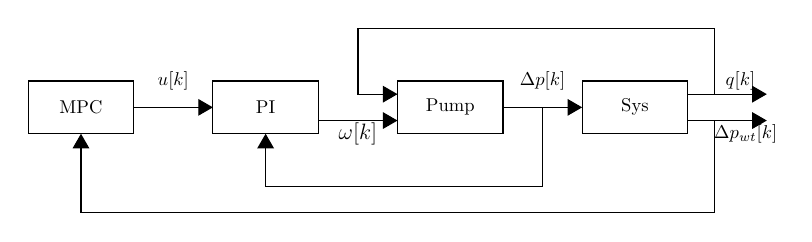
\begin{tikzpicture} [scale=0.67,transform shape]

\draw  (6,1) rectangle (8,0);
\node at (7,0.5) {Sys};

\draw  (-4.5,1) rectangle (-2.5,0);
\node at (-3.5,0.5) {MPC};

\draw  (2.5,1) rectangle (4.5,0);
\node at (3.5,0.5) {Pump};

\draw  (-1,1) rectangle (1,0);
\node at (0,0.5) {PI};

\draw[-triangle 60] (8,0.25) -- (9.5,0.25);
\draw[-triangle 60] (8,0.75) -- (9.5,0.75);
\draw[-triangle 60] (4.5,0.5) -- (6,0.5);
\draw[-triangle 60] (1,0.25) -- (2.5,0.25);
\draw[-triangle 60] (-2.5,0.5) -- (-1,0.5);
%\draw[-triangle 60] (-5.5,0.5) -- (-4.5,0.5);

\draw[-triangle 60] (5.25,0.5) -- (5.25,-1) -- (0,-1) -- (0,0);
\draw[-triangle 60] (8.5,0.75) -- (8.5,2) -- (1.75,2) -- (1.75,0.75) -- (2.5,0.75);
\draw[-triangle 60] (8.5,0.25) -- (8.5,-1.5) -- (-3.5,-1.5) -- (-3.5,0);

%\node at (-5.5,1) {$CP_{ref}$};
\node at (-1.75,1) {$u[k]$};
\node at (5.25,1) {$\Delta p[k]$};
\node at (1.75,0) {\large{$\omega[k]$}};
\node at (9.1,0) {${\Delta p_{wt}[k]}$};
\node at (9,1) {$q[k]$};

\end{tikzpicture}%
 
	%\caption{Cascade control structure with MPC and PI controllers.}
	%\label{fig:control_structure}
	\end{figure}}

% \begin{figure}[H]
% \centering
% 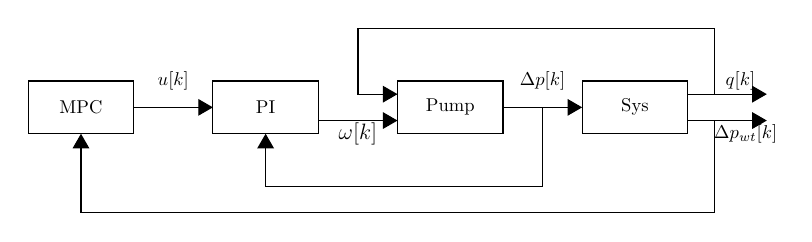
\begin{tikzpicture} [scale=0.67,transform shape]

\draw  (6,1) rectangle (8,0);
\node at (7,0.5) {Sys};

\draw  (-4.5,1) rectangle (-2.5,0);
\node at (-3.5,0.5) {MPC};

\draw  (2.5,1) rectangle (4.5,0);
\node at (3.5,0.5) {Pump};

\draw  (-1,1) rectangle (1,0);
\node at (0,0.5) {PI};

\draw[-triangle 60] (8,0.25) -- (9.5,0.25);
\draw[-triangle 60] (8,0.75) -- (9.5,0.75);
\draw[-triangle 60] (4.5,0.5) -- (6,0.5);
\draw[-triangle 60] (1,0.25) -- (2.5,0.25);
\draw[-triangle 60] (-2.5,0.5) -- (-1,0.5);
%\draw[-triangle 60] (-5.5,0.5) -- (-4.5,0.5);

\draw[-triangle 60] (5.25,0.5) -- (5.25,-1) -- (0,-1) -- (0,0);
\draw[-triangle 60] (8.5,0.75) -- (8.5,2) -- (1.75,2) -- (1.75,0.75) -- (2.5,0.75);
\draw[-triangle 60] (8.5,0.25) -- (8.5,-1.5) -- (-3.5,-1.5) -- (-3.5,0);

%\node at (-5.5,1) {$CP_{ref}$};
\node at (-1.75,1) {$u[k]$};
\node at (5.25,1) {$\Delta p[k]$};
\node at (1.75,0) {\large{$\omega[k]$}};
\node at (9.1,0) {${\Delta p_{wt}[k]}$};
\node at (9,1) {$q[k]$};

\end{tikzpicture}%
 
% %\caption{Cascade control structure with MPC and PI controllers.}
% %\label{fig:control_structure}
% \end{figure}

\end{frame}


\subsection{Model predictive control}

\begin{frame}{Controller}{Model predictive control}
\begin{itemize}
	\item<1-> Model predictive control 
	 	\begin{itemize}
	 	\item<1-> Take constraints into account	
	 	\item<1-> Take future prediction into account 
	 	\item<1-> Minimize the running cost of the system
	 	\end{itemize}
\end{itemize}
\onslide<1->{
\begin{figure}[H]
\centering
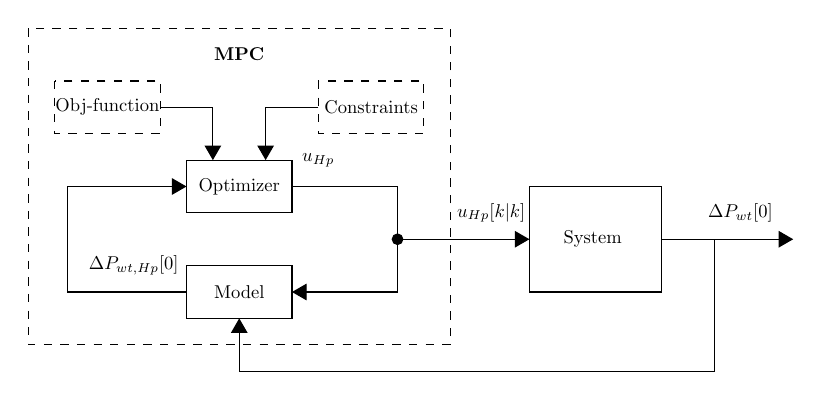
\begin{tikzpicture} [scale=0.67,transform shape]

\draw  (4.5,1.5) rectangle (7,-0.5);
%\node at (5.7,0.25) {Controller};
\node at (5.7,0.50) {System};

\draw  (-2,0) rectangle (0,-1);
\node at (-1,-0.5) {Model};

\draw  (-2,2) rectangle (0,1);
\node at (-1,1.5) {Optimizer};

\draw[dashed] (-5,4.5) rectangle (3,-1.5);

\draw[dashed]  (-4.5,3.5) rectangle (-2.5,2.5);
\node at (-3.5,3) {Obj-function};

\draw[dashed]  (0.5,3.5) rectangle (2.5,2.5);
\node at (1.5,3) {Constraints};

\draw[-triangle 60] (-4.25,0.75)-- (-4.25,1.5) -- (-2,1.5);
\draw[-triangle 60] (0.5,3)-- (-0.5,3) -- (-0.5,2);

\draw[-triangle 60] (2,0.5) -- (4.5,0.5);
\draw[-triangle 60] (7,0.5) -- (9.5,0.5);

\draw[-triangle 60] (-2.5,3)-- (-1.5,3) -- (-1.5,2);
%\draw[-triangle 60] (-5.5,0.5) -- (-4.5,0.5);

\draw[-triangle 60] (0,1.5) -- (2,1.5) -- (2,-0.5) -- (0,-0.5);
\draw[-triangle 60] (8,0.5) -- (8,-2) -- (-1,-2) -- (-1,-1);

\draw[-] (-2,-0.5) -- (-4.25,-0.5) -- (-4.25,0.75);

%\node at (-5.5,1) {$CP_{ref}$};
\node at (8.5,1) {$\Delta P_{wt}[0]$};
\node at (0.5,2) {$\pmb{u_{Hp}}$};
\node at (-3.0,0) {$\pmb{\Delta P_{wt,Hp}}[0]$};
%\node at (-2.5,2) {$\widetilde{e}$};
\node at (3.7762,1) {$\pmb{u_{Hp}}[k|k]$};
\node at (-1,4) {\textbf{MPC}};

%\draw  (-4.25,0.5) ellipse (0.25 and 0.25);
\draw[fill]  (2,0.5) ellipse (0.1 and 0.1);
\end{tikzpicture}%
 
%\caption{The block of MPC algorithm \cite{Camacho2007}.}
%\label{mpc_structure}
\end{figure}}
\end{frame}


% \onslide<2->{
% \begin{equation}
% \Upsilon(\bm{u}[k],\bm{q_p}[k],c_p[k]) = \frac{1}{\eta} \sum_{i=1}^{H_p-1} \Big( \bm{u^T}[k+i|k] \cdot  \bm{q_{p}}[k+i|k]\Big)\cdot c_p[k+i|k]
% \end{equation}}


\begin{frame}{Controller}{Model predictive control}
\onslide<1->{
\begin{equation}
\Upsilon(u[k],q_p[k],c_p[k]) = \frac{1}{\eta} \sum_{i=0}^{H_p-1} \Big( \underbrace{u^T[k+i|k] \cdot  q_{p}[k+i|k]}_{\text{Hydraulic Power}}\Big)\cdot c_p[k+i|k]
\end{equation}}

\begin{itemize}
	\item<1-> Model predictive control 
	 	\begin{itemize}
	 	\item<1-> Minimize the running cost of the system
	 	\end{itemize}
	\item<2-> Reformulation of the objective function 
	 	\begin{itemize}
	 	\item<2-> Formulating as a standard optimization problem 
	 	\end{itemize}
	\item<2-> Reformulation of the constraints 
	 	\begin{itemize}
	 	\item<2-> All constraints depend on the control input 
	 	\item<2-> Set up as a linear matrix inequality 
	 	\end{itemize}
\end{itemize}

\end{frame}

\begin{frame}{Controller}{Model predictive control}
\begin{equation}
	\Upsilon(\pmb{\hat{u}_{Hp}}) = \frac{1}{\eta}\bigg( \frac{1}{2} \pmb{\hat{u}_{{Hp}}^{T}} \pmb{R} \pmb{\hat{u}_{Hp}} + \pmb{b} \pmb{\hat{u}_{Hp}} + c \bigg)
\end{equation}
\begin{itemize}
	\item<1-> Convexity 
	 	\begin{itemize}
	 	\item<1-> Ensuring convexity 
	 	\item<1-> Hessian of $\Upsilon(\pmb{\hat{u}_{Hp}}) \ge 0$ 
	 	\item<1-> $\pmb{R} \succeq 0$
	 	\end{itemize}
\end{itemize}
\end{frame}
%%%%%%%%%%%%%%%%
\section{Implementation}
%%%%%%%%%%%% MID WAY AGENDA %%%%%%%%%%%%%%
%\begin{frame}<beamer>
%\frametitle{Thomas Holm Pilgaard}
%\tableofcontents[currentsection]
%\end{frame}
%%%%%%%%%%%% MID WAY AGENDA %%%%%%%%%%%%%%

% \begin{frame}{Parameter identification results}{Wrong measurement data}

% \begin{itemize}
% 	 	\item<1-> Measurement data is not around the operating point
% 	 	\item<1-> Steady state error in the model
% 	 	\end{itemize}

% \begin{figure}[H]
%    \centering
%     % This file was created by matlab2tikz.
%
%The latest updates can be retrieved from
%  http://www.mathworks.com/matlabcentral/fileexchange/22022-matlab2tikz-matlab2tikz
%where you can also make suggestions and rate matlab2tikz.
%
\definecolor{mycolor1}{rgb}{0.00000,0.44700,0.74100}%
\definecolor{mycolor2}{rgb}{0.85000,0.32500,0.09800}%
%
\begin{tikzpicture}

\begin{axis}[%
scaled y ticks = false,
 y tick label style={/pgf/number format/fixed,
/pgf/number format/1000 sep = \thinspace}, % Optional if you want to replace comma as the 1000 separator 
width=3.8in,
height=1in,
at={(1.011in,0.642in)},
scale only axis,
xmin=0,
xmax=500,
xlabel style={font=\color{white!15!black}},
xlabel={Time [min]},
ymin=-0.005,
ymax=0.01,
ylabel style={font=\color{white!15!black}},
ylabel={Pressure [bar]},
axis background/.style={fill=white},
%title style={font=\bfseries},
%title={Node WT},
xmajorgrids,
ymajorgrids,
legend style={legend cell align=left, align=left, draw=white!15!black}
]
\addplot [color=mycolor1]
  table[row sep=crcr]{%
0.000833333333333333	-0.000536486839485997\\
0.0508333333333333	-0.000992361717296275\\
1.07083333333333	-0.000214590456297223\\
1.15416666666667	-0.000472107562845242\\
1.86083333333333	0.000207354802741866\\
2.23	-4.84223233562925e-05\\
3.3075	0.000626690091107954\\
3.38583333333333	0.00026912410870214\\
4.09666666666667	0.000805908077422438\\
4.44416666666667	0.000669319612141839\\
5.46916666666667	0.00114433427489903\\
5.94	0.00103123554567336\\
6.4975	0.00157758940687817\\
6.65083333333333	0.00135139194838989\\
7.67916666666667	0.00184728637653113\\
7.8475	0.00162804883988631\\
8.4725	0.0021700527499505\\
9.06583333333333	0.00190383574114041\\
9.86583333333333	0.00231708109796219\\
10.0333333333333	0.00219441247628542\\
10.6625	0.00268682694352837\\
11.0708333333333	0.00237276047235473\\
11.9325	0.00287561482232949\\
12.2391666666667	0.00264245744206168\\
13.1041666666667	0.00312878197772765\\
13.3541666666667	0.00290519448994932\\
13.9108333333333	0.00333583965122845\\
14.45	0.00299306350267163\\
15.3741666666667	0.00356551707060934\\
15.4558333333333	0.00319925118595282\\
16.3025	0.00368905568249719\\
17.1833333333333	0.00390046330714998\\
17.2666666666667	0.00343501853685101\\
17.7641666666667	0.00356899703145931\\
18.6308333333333	0.00404227171378015\\
19.0908333333333	0.00377257474405045\\
19.6383333333333	0.00423018960235598\\
19.9341666666667	0.00388045353190596\\
20.8775	0.00436242811647393\\
21.1391666666667	0.00397441247625356\\
22.0441666666667	0.0044946666306203\\
22.67	0.00417973016928958\\
23.1425	0.00461211531109033\\
23.3208333333333	0.00417886017903019\\
24.1791666666667	0.00470868422599441\\
24.2483333333333	0.00433110846838648\\
25.3183333333333	0.00482178295526413\\
25.3691666666667	0.00455295597579951\\
25.79	0.0049087819777299\\
26.8133333333333	0.00458514561404404\\
27.0483333333333	0.0050358005505473\\
27.8891666666667	0.00470172430424899\\
28.3883333333333	0.00516716907457639\\
29.2941666666667	0.00481656301394655\\
29.7325	0.0051523792407011\\
29.7625	0.00490095206570235\\
30.6466666666667	0.00583619155747787\\
30.9566666666667	0.00560738412834215\\
31.9533333333333	0.00616591785262703\\
32.1408333333333	0.00594842029645977\\
32.8883333333333	0.00647563437269132\\
33.1991666666667	0.00620158745181247\\
34.0508333333333	0.00664006252517314\\
34.1708333333333	0.00652087386437759\\
35.2375	0.00694281912341242\\
35.4483333333333	0.00672184160628152\\
36.2408333333333	0.00713334698266412\\
36.4483333333333	0.00697674874195404\\
37.3158333333333	0.00742740367857099\\
37.6408333333333	0.00707940758862836\\
38.46	0.00757269204601703\\
38.6225	0.00731604492973477\\
39.6466666666667	0.00780062948502976\\
39.7975	0.00756138217316223\\
40.6383333333333	0.0079667976179849\\
40.7991666666667	0.00765708109780693\\
41.6566666666667	0.00818690514487348\\
41.8908333333333	0.00782411922099303\\
42.715	0.00827129419660654\\
43.3516666666667	0.00802073701192969\\
43.67	0.00845747210482846\\
44.3908333333333	0.0085496910686516\\
44.6391666666667	0.00811904590741509\\
45.4466666666667	0.00827303417712531\\
46.12	0.00876283867381748\\
46.3391666666667	0.0084157125740376\\
47.34	0.00886201755934056\\
47.4641666666667	0.00854534111753087\\
48.0433333333333	0.00904210553595707\\
48.7341666666667	0.00868540954363657\\
49.5266666666667	0.00909604492984502\\
49.745	0.00882373798954179\\
50.2425	0.00916390416738298\\
50.8483333333333	0.00889420719768171\\
51.74	0.00929005275006607\\
51.8875	0.00899686604425372\\
52.3775	0.00934312215351842\\
52.9958333333333	0.00912388461709955\\
53.6241666666667	0.0094927604723694\\
54.0066666666667	0.00912823456810659\\
55.0375	0.00955452977834743\\
55.165	0.0092430732779349\\
56.1508333333333	0.00968241834136736\\
56.4716666666667	0.00932572234918329\\
57.2933333333333	0.00978159722704962\\
57.5741666666667	0.0097902971291433\\
57.9783333333333	0.00945274092208596\\
58.5308333333333	0.00950929028662136\\
59.2725	0.0098451065133759\\
59.645	0.009886866044144\\
60.4433333333333	0.00909865490045834\\
61.0316666666667	0.00887158745175616\\
61.1091666666667	0.00942490123472912\\
61.9116666666667	0.00928483280862343\\
62.6825	0.0087697985954492\\
62.86	0.00909604492984502\\
63.8058333333333	0.00856796086343369\\
63.9925	0.00886897748114283\\
64.995	0.00851315147931477\\
65.1666666666667	0.00872716907451836\\
65.7458333333333	0.00828695402080944\\
66.3466666666667	0.00856883085373288\\
66.6825	0.00814340563367753\\
67.6433333333333	0.00840266272052763\\
68.0608333333333	0.00795896770581524\\
68.4358333333333	0.00827390416728808\\
69.1133333333333	0.00795374776472503\\
69.5491666666667	0.00822692469517965\\
69.5725	0.00784586897667626\\
70.65	0.00811034600502585\\
71.2266666666667	0.00772494033525394\\
71.6541666666667	0.00798419742237687\\
72.7375	0.00754050240778954\\
73.01	0.00791720817486526\\
73.6141666666667	0.00744828344392094\\
74.1575	0.00781106936782412\\
74.9383333333333	0.00738390416730685\\
75.115	0.00766665099071136\\
76.005	0.00719424629820654\\
76.65	0.00756399214379828\\
76.955	0.00711942713888906\\
77.415	0.00746307327787012\\
78.0891666666667	0.00708201755936673\\
78.2833333333333	0.00740913388382299\\
78.9216666666667	0.00695325900600215\\
79.5525	0.0073247448319876\\
80.4225	0.00694977904523743\\
80.7716666666667	0.00725253564354493\\
81.3908333333333	0.00688365978818413\\
82.4541666666667	0.00680275069711346\\
82.5333333333333	0.00718293642545408\\
82.8233333333333	0.00713421697295193\\
83.1758333333333	0.0067183616453463\\
84.1275	0.00706809771546664\\
84.8033333333333	0.00658960309225452\\
84.8933333333333	0.00701241834125317\\
85.9116666666667	0.0065565434635005\\
86.6733333333333	0.00652870377638241\\
86.8425	0.00695325900604761\\
87.67	0.00687843984666191\\
88.1383333333333	0.00650869400120659\\
88.2233333333333	0.0068323303650573\\
89.1141666666667	0.00642778491038602\\
89.2983333333333	0.0067879608633007\\
90.3308333333333	0.00538205665992568\\
90.4525	0.0055621446368264\\
91.4575	0.00500187093206254\\
91.7041666666667	0.00525851804817425\\
92.54	0.0045085864743783\\
92.7266666666667	0.00477045353203497\\
93.6683333333333	0.0041240507948601\\
93.8883333333333	0.00454947601482449\\
94.51	0.00382999409893049\\
94.8683333333333	0.00419104004230351\\
95.8275	0.00350983769623102\\
95.955	0.0038752335908271\\
96.76	0.00318794131306963\\
97.1091666666667	0.00357421697282238\\
98.0425	0.00285995499820051\\
98.1075	0.00319490123468999\\
99.0458333333333	0.00267899703131892\\
99.4766666666667	0.00293564414743062\\
99.8283333333333	0.0024319198074068\\
100.315833333333	0.00281993544775791\\
101.033333333333	0.00216657278884899\\
101.403333333333	0.00234405079478396\\
102.028333333333	0.00192471550636814\\
102.680833333333	0.00216396281815609\\
103.588333333333	0.001644578654134\\
103.755	0.00201258451930929\\
104.6	0.00147493056018679\\
104.76	0.00184032645473739\\
105.77	0.00114259429432199\\
106.074166666667	0.00161673896674305\\
106.840833333333	0.00112432449958537\\
107.080833333333	0.00133486213409245\\
107.939166666667	0.000972076210166539\\
108.080833333333	0.00118087386405254\\
108.774166666667	0.000732828898560495\\
109.131666666667	0.00108604492980934\\
110.001666666667	0.000624080120462653\\
110.216666666667	0.000841577676476427\\
111.150833333333	0.000406582564357938\\
111.563333333333	0.000743268781309356\\
112.415	0.000279563991478007\\
112.455833333333	0.000609290286672642\\
112.814166666667	0.000178645125436139\\
113.62	0.000489231635367599\\
114.365	4.81465916778168e-05\\
115.125833333333	0.000368302994468231\\
115.4075	-0.000117151550909925\\
116.065	0.00029870377637739\\
116.373333333333	-0.000248520074990169\\
116.908333333333	0.000155155389177292\\
117.788333333333	-0.000298109517950673\\
118.435	2.98767968957142e-05\\
118.604166666667	-0.000388588501198189\\
119.695833333333	-0.000419908149149217\\
119.880833333333	0.000413542486114735\\
120.1675	0.000105565946603325\\
121.139166666667	0.000501411498828513\\
121.283333333333	0.000227364577756392\\
121.854166666667	0.000693679338462552\\
122.6025	0.000460521958063995\\
123.380833333333	0.000961636327417678\\
123.4625	0.000743268781309356\\
124.504166666667	0.00114694424531767\\
124.9125	0.000882467217309155\\
125.5225	0.00139924141050191\\
125.796666666667	0.00107560504699226\\
126.219166666667	0.00148015050157259\\
127.1175	0.00161847894747784\\
127.699166666667	0.00128179273038999\\
128.011666666667	0.00140707132280798\\
128.468333333333	0.00170286799931323\\
129.098333333333	0.00156279957299152\\
129.788333333333	0.00180204688484768\\
130.3225	0.00165849849767032\\
130.539166666667	0.00198561482230847\\
131.248333333333	0.00178203710974006\\
132.12	0.0020352042650416\\
132.608333333333	0.00196995499810558\\
133.1375	0.00217962264219981\\
133.405833333333	0.0019525551938273\\
134.408333333333	0.00230316125424683\\
134.744166666667	0.00216309282819797\\
135.503333333333	0.00237363046250043\\
135.891666666667	0.00217788266171513\\
136.6675	0.00253457865395607\\
137.1925	0.00258851804782129\\
137.335833333333	0.00230490123493614\\
137.84	0.00238494033595775\\
138.808333333333	0.00276425607384002\\
139.506666666667	0.00246062948502872\\
139.593333333333	0.00275642616232975\\
140.186666666667	0.00245105959292008\\
140.965	0.00289475460775751\\
141.4925	0.00255110846823076\\
142.175833333333	0.00290171452942335\\
142.408333333333	0.00265115734435999\\
143.1275	0.00297740367904002\\
143.38	0.00266420719816556\\
144.2375	0.0030243831514213\\
144.466666666667	0.00270596672902461\\
145.256666666667	0.00311747210483876\\
146.374166666667	0.0027546861811857\\
146.4575	0.00318794131306963\\
147.056666666667	0.00280166565411268\\
147.330833333333	0.00322970084361035\\
148.071666666667	0.0028773548032746\\
148.791666666667	0.00325145059977107\\
149.050833333333	0.00287213486170688\\
149.860833333333	0.00340369888939453\\
149.893333333333	0.00325058060979021\\
150.83	0.0039135131604667\\
151.1775	0.00428847894744426\\
151.945	0.00371689536958687\\
152.315833333333	0.00378997454862433\\
153.1525	0.00426411922152287\\
153.238333333333	0.0039657125741883\\
154.2325	0.00442506741263746\\
154.315833333333	0.00405358158662925\\
155.198333333333	0.00460341540850781\\
155.4825	0.00426324923136011\\
156.505	0.00465735480250945\\
156.8	0.00451641638672985\\
157.609166666667	0.00493749165510739\\
157.6975	0.00461820524259342\\
158.700833333333	0.00503754053132756\\
158.765	0.00485658256478703\\
159.806666666667	0.00519326878155656\\
159.993333333333	0.00490617200701994\\
160.8075	0.0053516070025012\\
161.3525	0.00505581032551848\\
161.619166666667	0.00547688559498742\\
162.095833333333	0.00520022870363167\\
162.490833333333	0.00565175362988841\\
163.600833333333	0.00534203710998331\\
163.851666666667	0.00566654346388308\\
164.450833333333	0.00538466663091416\\
165.16	0.00582575167444478\\
165.6125	0.00545426584843657\\
166.054166666667	0.00589361091196002\\
166.581666666667	0.00563435382495077\\
167.184166666667	0.0059571201987524\\
167.7825	0.00566654346338287\\
168.3725	0.00599713974860382\\
168.805	0.00571700289646064\\
169.3875	0.00614677806805734\\
169.758333333333	0.00585620133305161\\
170.738333333333	0.00620854737334188\\
171.451666666667	0.00594059038461413\\
171.8825	0.00635209576097399\\
172.335833333333	0.00599365978804374\\
172.491666666667	0.00630511628886556\\
173.075833333333	0.00603280934827811\\
174.026666666667	0.00644257474422151\\
174.6175	0.00615721795001041\\
175.04	0.0064643245002458\\
175.360833333333	0.00618331765789439\\
175.693333333333	0.00655741345389065\\
176.583333333333	0.00622681716853325\\
177.395	0.00659917298493158\\
177.9325	0.00628684649394702\\
178.433333333333	0.00665920231057275\\
178.843333333333	0.0062868464943563\\
179.63	0.00661570279925176\\
179.706666666667	0.00660178295482867\\
180.4625	0.00593711042378121\\
180.76	0.00617635773527357\\
181.635833333333	0.00576311237872464\\
181.86	0.00597625998365177\\
182.786666666667	0.0054264261610911\\
183.0075	0.0058040019189662\\
183.839166666667	0.00530549752032815\\
184.069166666667	0.00563696379589378\\
184.88	0.00514367933859607\\
185.18	0.00543599605383636\\
186.074166666667	0.0049818611570004\\
186.4975	0.00529157767649625\\
187.1575	0.0048765923396218\\
187.725833333333	0.00480873310197015\\
188.004166666667	0.00511931961240183\\
188.5525	0.00504363046255779\\
189.555	0.00466518471465636\\
190.189166666667	0.00488964219260883\\
190.2725	0.00450249654303438\\
191.14	0.00476871355175494\\
191.398333333333	0.00445029712963109\\
191.813333333333	0.0046173352532492\\
191.844166666667	0.00437547797045003\\
193.7	0.00418147015033131\\
193.783333333333	0.00458949556563087\\
194.255	0.00444594717845352\\
194.815833333333	0.00417364023841177\\
195.985833333333	0.00437982792121833\\
196.06	0.00404836164551629\\
196.933333333333	0.00386914365898296\\
197.0175	0.00434067836112038\\
197.603333333333	0.00392917298521528\\
198.156666666667	0.00427629908507474\\
198.6375	0.00425802929006526\\
198.944166666667	0.00387784356206571\\
199.669166666667	0.00419191003314839\\
199.9775	0.0037664848125019\\
200.915	0.00414928051180827\\
201.564166666667	0.0037725747443233\\
201.768333333333	0.004033571811749\\
202.4675	0.00367687581978092\\
202.929166666667	0.00405184160612183\\
203.621666666667	0.00359161677714613\\
204.505	0.00365251609299552\\
204.585833333333	0.00399094229022698\\
205.1475	0.0039865923394132\\
205.626666666667	0.00354985724683278\\
206.756666666667	0.00389002342470807\\
207.026666666667	0.0035254975203657\\
207.9675	0.00351505763754861\\
208.286666666667	0.00395875265261342\\
209.04	0.00348634796044965\\
209.41	0.00380650436303544\\
209.411666666667	0.003812594294584\\
209.891666666667	0.00285473505736039\\
210.5625	0.00350287777404222\\
211.525833333333	0.00307745255462354\\
211.723333333333	0.00338542909456695\\
212.393333333333	0.00294173407995689\\
212.790833333333	0.00327059038417023\\
213.818333333333	0.00284951511602007\\
213.905833333333	0.00311660211476696\\
214.634166666667	0.00270422674806245\\
215.219166666667	0.00293738412837005\\
215.784166666667	0.00256589830254374\\
216.515833333333	0.00286343495948817\\
217.0375	0.00246323945660837\\
217.864166666667	0.00236145059951699\\
218.144166666667	0.0027146666312888\\
218.6975	0.00267116712001329\\
219.034166666667	0.00225009185086268\\
219.7325	0.00253892860536102\\
220.304166666667	0.0021256832485847\\
220.466666666667	0.00253805861560753\\
221.120833333333	0.00209610358141393\\
222.034166666667	0.00237015050169025\\
222.084166666667	0.00201867445101701\\
223.091666666667	0.0022883714202067\\
223.623333333333	0.0018377164846584\\
224.093333333333	0.0022266021144674\\
224.74	0.00184206643579049\\
225.549166666667	0.00215091296530549\\
225.881666666667	0.00178029712923265\\
226.07	0.00207783378617708\\
226.785833333333	0.00165066858606909\\
227.296666666667	0.00204651413822607\\
227.7325	0.0016463186351189\\
228.655833333333	0.00197256496916229\\
228.861666666667	0.00160542909446808\\
229.399166666667	0.00192471550730038\\
229.7125	0.00151495011044749\\
231.155	0.00193602537959808\\
231.414166666667	0.00150712019839151\\
231.775833333333	0.00181248676798308\\
232.34	0.00143404101949049\\
232.639166666667	0.00137227171379667\\
232.999166666667	0.00178029712941456\\
234.129166666667	0.00135574189988578\\
234.308333333333	0.00173940758867279\\
235.156666666667	0.00166371843987466\\
235.661666666667	0.00129484258380902\\
236.54	0.00165414854672012\\
236.575	0.00123481325857715\\
237.670833333333	0.0016002091528549\\
237.693333333333	0.00126178295512322\\
238.505	0.00155931961184028\\
239.070833333333	0.00119044375650222\\
239.6075	0.00117391394240944\\
239.890833333333	0.00195429517460756\\
240.770833333333	0.00144361091214482\\
240.981666666667	0.00188034600531641\\
241.724166666667	0.00157149947530119\\
242.4275	0.00199170475401619\\
243.393333333333	0.00162021892778061\\
243.575833333333	0.00209262362021721\\
243.964166666667	0.00176898725625282\\
244.370833333333	0.00219876242762215\\
245.205	0.00190557572271931\\
245.478333333333	0.00228489146019233\\
245.949166666667	0.00199866467600035\\
246.354166666667	0.0023849403364125\\
247.235	0.00207261384506413\\
247.829166666667	0.00248933916312812\\
248.329166666667	0.00208044375707463\\
248.8375	0.00259895793068385\\
249.189166666667	0.00220050240808409\\
249.7075	0.00261461775579623\\
250.246666666667	0.00224835187026433\\
251.099166666667	0.002765996054211\\
251.9675	0.00242582987633572\\
252.328333333333	0.00280775558525197\\
252.44	0.00281210553670239\\
253.056666666667	0.00240843007194375\\
253.8975	0.0025180488399997\\
253.983333333333	0.00291563437293693\\
254.624166666667	0.00255023847834085\\
254.914166666667	0.00293651413852562\\
255.990833333333	0.00264158745266062\\
256.754166666667	0.00305570279941779\\
256.984166666667	0.0026502873544246\\
257.270833333333	0.0031157321244223\\
258.0975	0.00271988657240176\\
258.724166666667	0.00306875265308694\\
259.311666666667	0.00276686604410091\\
260.065833333333	0.00315053173316077\\
260.6775	0.00278165587832295\\
260.901666666667	0.00321230103949123\\
261.615833333333	0.0028521250865538\\
261.699166666667	0.0032523205899793\\
262.6825	0.00324884062919185\\
262.825	0.00284429517467974\\
263.676666666667	0.00289301462684083\\
264.419166666667	0.00332017982713072\\
265.101666666667	0.00291911433363343\\
265.186666666667	0.00331930983696797\\
265.890833333333	0.00294956399196739\\
266.551666666667	0.00336280934869823\\
266.7825	0.00302699312186409\\
266.865	0.00341587875230974\\
268.590833333333	0.00303569302376448\\
268.773333333333	0.00344545841975336\\
269.238333333333	0.00289997454923427\\
269.3225	0.00351418764734039\\
270.565	0.00322883085349307\\
270.881666666667	0.00287735480300175\\
271.269166666667	0.00315053173366099\\
271.513333333333	0.00268073701262214\\
272.8425	0.00299828344431038\\
272.875833333333	0.00259547797007829\\
273.335833333333	0.00296000387442068\\
274.323333333333	0.00228402146984767\\
275.316666666667	0.00281123554599393\\
275.539166666667	0.00238494033577584\\
275.8475	0.00265376731539395\\
276.171666666667	0.00227793153734414\\
277.071666666667	0.00258764805674903\\
277.536666666667	0.00224139194777993\\
278.160833333333	0.00254066858495892\\
278.6025	0.00216570279816328\\
279.3575	0.00243539976671631\\
279.738333333333	0.00203607425481782\\
280.2075	0.00237102049085255\\
281.035833333333	0.00195429517324332\\
281.131666666667	0.00184293642504375\\
281.3275	0.00231447112599885\\
282.463333333333	0.00179769693339725\\
282.5475	0.00229533134150874\\
283.586666666667	0.00171765783314871\\
283.935	0.00211872332555461\\
284.645	0.00166284844871147\\
285.168333333333	0.00209871355162936\\
285.479166666667	0.00199083476344417\\
286.078333333333	0.00159150925018142\\
286.728333333333	0.00191253564133835\\
287.343333333333	0.00153669986619892\\
287.755833333333	0.00145057083344685\\
287.929166666667	0.00191340563295629\\
288.8725	0.00142099116554849\\
289.056666666667	0.00180291687473759\\
289.9725	0.00175854737252625\\
290.835833333333	0.00126526291604709\\
290.9875	0.0017776871578349\\
292.059166666667	0.00133486213416066\\
292.293333333333	0.00166458842949173\\
292.654166666667	0.00127396281831128\\
293.415833333333	0.00162891882945364\\
293.560833333333	0.00114694424554504\\
294.574166666667	0.00117130397237591\\
295.185833333333	0.00154539976864503\\
295.633333333333	0.00160281912347958\\
296.4	0.00115564414871873\\
296.49	0.00151234013973184\\
297.338333333333	0.00109822479324752\\
298.370833333333	0.00142012117556764\\
298.639166666667	0.000892907099921597\\
298.723333333333	0.00154191980699356\\
299.735	0.000878987257226557\\
299.818333333333	0.00160716907402052\\
300.2225	0.00102775558533498\\
301.149166666667	0.0011573841273162\\
301.861666666667	0.00158628930829539\\
302.311666666667	0.00121045353261028\\
302.393333333333	0.00160803906418326\\
303.900833333333	0.00101470573289365\\
304.184166666667	0.00165153857586806\\
304.766666666667	0.00129310260289234\\
304.9575	0.00169938803782092\\
305.860833333333	0.00135835187073784\\
306.335	0.00171765783287586\\
306.685	0.00177681716739929\\
307.318333333333	0.0012121935118444\\
308.164166666667	0.00179334698231064\\
308.2475	0.00138619155803785\\
308.95	0.00183597650328697\\
309.165833333333	0.00146362068779812\\
310.108333333333	0.00147145059880817\\
310.474166666667	0.00184119644417255\\
311.023333333333	0.00149929028583533\\
311.6425	0.00185511628759517\\
311.924166666667	0.00194907523108444\\
311.993333333333	0.00149059038329828\\
313.476666666667	0.00152712997440861\\
313.768333333333	0.00192645548603426\\
314.201666666667	0.00156366956369997\\
315.143333333333	0.00196299507532562\\
315.601666666667	0.00162717884885527\\
316.098333333333	0.00196038510520115\\
316.8975	0.00203520426520075\\
317.2575	0.00158628930820445\\
317.854166666667	0.00161151902501619\\
318.255833333333	0.00198648481226658\\
319.21	0.0014862404323026\\
319.298333333333	0.00210306350171553\\
320.500833333333	0.00161412899568635\\
320.69	0.00200040465523448\\
320.839166666667	0.00163413877115776\\
320.9175	0.00203172430291264\\
322.065833333333	0.0016323987901956\\
322.149166666667	0.00202824434244352\\
323.178333333333	0.0016323987898318\\
323.925833333333	0.00202998432267808\\
324.149166666667	0.00160890905507362\\
324.2325	0.00203694424443487\\
325.323333333333	0.0016332687808131\\
325.594166666667	0.00206739390258694\\
327.071666666667	0.00159498921119625\\
327.155	0.00198735480115605\\
327.753333333333	0.00201780445994476\\
328.114166666667	0.00161064903530818\\
328.758333333333	0.00196473505583303\\
329.06	0.00163413877170346\\
329.755	0.00162717884949191\\
329.841666666667	0.00232839097042191\\
330.665	0.00204042420526779\\
331.738333333333	0.00244322967936345\\
331.764166666667	0.00213786311013568\\
332.288333333333	0.00259199800801756\\
332.9175	0.00232143104730088\\
333.6775	0.00275903613190852\\
333.9975	0.00239712019846369\\
335.015833333333	0.00287735480150107\\
335.255	0.00256241834084679\\
336.065	0.00306614268118896\\
336.334166666667	0.00272945646373732\\
337.068333333333	0.0031218220560618\\
337.800833333333	0.00284603515455049\\
338.108333333333	0.00326972039355272\\
338.54	0.00297392371793424\\
338.9075	0.00332626975831549\\
339.575833333333	0.00305570279878115\\
340.0975	0.00345241834173753\\
340.745	0.0031018122809542\\
341.628333333333	0.00351853759838154\\
341.668333333333	0.00322361091210727\\
342.7225	0.00372472528223401\\
343.404166666667	0.00327842029518027\\
343.478333333333	0.00369775558482392\\
344.9075	0.00385522381501463\\
344.936666666667	0.00334714952322206\\
345.384166666667	0.00341065881128774\\
345.468333333333	0.00383434405047187\\
346.135	0.00347764805718502\\
346.8675	0.00392569302374572\\
347.3175	0.00354463730471938\\
348.179166666667	0.00405793153785229\\
348.426666666667	0.00359596672832371\\
349.1075	0.00407881130266791\\
349.726666666667	0.00408403124555438\\
349.755	0.00358552684637065\\
350.864166666667	0.00372646526310522\\
351.400833333333	0.00421452977860785\\
352.269166666667	0.00420930983772226\\
352.418333333333	0.00383434404983522\\
352.825833333333	0.00424323945752579\\
353.6225	0.00383173408025644\\
354.305	0.00387436360050518\\
354.7875	0.00436938803812841\\
355.030833333333	0.00381607425496217\\
355.1125	0.00431283867336564\\
356.963333333333	0.00396136262323811\\
357.045833333333	0.00438939781460025\\
357.815	0.00399094229086362\\
357.995	0.00430152880052223\\
358.451666666667	0.00446247699209155\\
358.741666666667	0.00388915343381772\\
359.403333333333	0.00435894815517489\\
360.095833333333	0.00387523359048604\\
360.716666666667	0.00424671941672163\\
361.505	0.00375343495860538\\
361.5725	0.00413623066004906\\
362.488333333333	0.00373516516364138\\
362.871666666667	0.00404836164442489\\
363.680833333333	0.00363424629866817\\
364.046666666667	0.00395179273081116\\
364.771666666667	0.00352114756841505\\
365.053333333333	0.00385696379606774\\
365.450833333333	0.0034759080768595\\
366.105833333333	0.00382912410813109\\
366.700833333333	0.0034411084688941\\
367.151666666667	0.00373429517438811\\
368.115	0.00331582987581673\\
368.621666666667	0.00364642616312953\\
368.876666666667	0.00324797063848341\\
369.27	0.00319142127372064\\
369.4375	0.0036029266504443\\
370.769166666667	0.00352375754008566\\
370.985	0.00317576144869922\\
372.423333333333	0.00312791198711014\\
372.441666666667	0.00346720817532291\\
372.683333333333	0.003493307881206\\
373.478333333333	0.00303830299334326\\
374.13	0.00291041442995951\\
374.654166666667	0.00335671941683134\\
375.045	0.0033193098361949\\
375.143333333333	0.00298001364889164\\
376.146666666667	0.00288692469529227\\
376.610833333333	0.00331756985668794\\
377.888333333333	0.00324623065715744\\
378.021666666667	0.00287039488092664\\
378.129166666667	0.00280775558429699\\
378.280833333333	0.00321752097996754\\
379.829166666667	0.003156621664391\\
380.155	0.0028442951733155\\
380.603333333333	0.00317315147848379\\
381.168333333333	0.00276686604310047\\
381.405	0.0031018122811361\\
381.488333333333	0.00268508696225357\\
382.704166666667	0.00310355226073401\\
383.408333333333	0.00262853759767272\\
383.6025	0.00262157767591592\\
383.683333333333	0.003100072300083\\
385.525833333333	0.00305222283658399\\
385.653333333333	0.00261983769549946\\
385.7975	0.00260156790044451\\
386.628333333333	0.00294086408829347\\
387.2225	0.0029713137461727\\
387.245833333333	0.00257111824292909\\
388.753333333333	0.00255632840861612\\
388.846666666667	0.00292172430425812\\
389.454166666667	0.00293042420597661\\
390.058333333333	0.00246236946439925\\
390.344166666667	0.00228750142931634\\
390.585833333333	0.00277469595411052\\
391.265833333333	0.00261200778385277\\
392.271666666667	0.00223965196654494\\
392.604166666667	0.0025980879401573\\
393.464166666667	0.00208392371695258\\
393.544166666667	0.00245714952433222\\
394.4	0.00207783378581329\\
394.961666666667	0.00241538999315484\\
395.445	0.00197430494844188\\
395.774166666667	0.00230403124286344\\
395.988333333333	0.00190818569152501\\
397.4675	0.00176637728453674\\
397.545	0.00223791198585563\\
398.365	0.00212568324803901\\
398.661666666667	0.00173940758839994\\
399.241666666667	0.00203259429425774\\
400.021666666667	0.00160716907438431\\
400.294166666667	0.00197343495837007\\
400.805833333333	0.00162108891880738\\
401.275	0.00194820524237688\\
402.045	0.00140011140055098\\
402.3325	0.00184467640555117\\
402.779166666667	0.00151495011040201\\
404.080833333333	0.0013975014307903\\
404.159166666667	0.00181944668919418\\
404.886666666667	0.00171765783269397\\
404.919166666667	0.00132181228090079\\
405.76	0.00172287777476189\\
406.674166666667	0.00126178295557797\\
407.135833333333	0.00121306350200716\\
407.583333333333	0.00159933916237381\\
407.891666666667	0.00157845939619396\\
408.323333333333	0.00107212508572734\\
409.380833333333	0.00114172430438661\\
409.74	0.0015497497203683\\
410.174166666667	0.00109300485127055\\
410.255833333333	0.00151930006176147\\
411.514166666667	0.00104776536089733\\
411.856666666667	0.00143926096042155\\
412.4075	0.000963376307379388\\
412.975	0.00138706154747301\\
413.7275	0.0013600918509724\\
414.178333333333	0.000969466240519565\\
414.638333333333	0.0013766216645195\\
415.12	0.000898127042353314\\
416.009166666667	0.00123655323931192\\
416.031666666667	0.000892907100285389\\
417.148333333333	0.00130615245651601\\
417.5325	0.000813737990108657\\
417.906666666667	0.00125482303282073\\
418.781666666667	0.000898127041443819\\
418.910833333333	0.00120088363991049\\
419.2925	0.000810258028275293\\
419.920833333333	0.000842447666570975\\
420.500833333333	0.00120523359145185\\
421.184166666667	0.00128092274097756\\
421.975833333333	0.000805038087116863\\
423.079166666667	0.000730218927844847\\
423.163333333333	0.00130615245769836\\
423.4575	0.00127048285738741\\
423.511666666667	0.000734568878203876\\
424.706666666667	0.000770238478514818\\
425.04	0.00122263339470695\\
425.976666666667	0.00120523359054235\\
426.383333333333	0.000762408566322426\\
427.003333333333	0.000799818146413181\\
427.086666666667	0.00128092273979523\\
428.054166666667	0.000677149524096907\\
428.233333333333	0.00123220328749771\\
429.253333333333	0.00115042420601416\\
429.2825	0.000734568879386222\\
430.565833333333	0.000720649036782137\\
430.65	0.00127483280920164\\
431.350833333333	0.000810258029002892\\
431.44	0.00115129419672261\\
432.860833333333	0.00115129419745021\\
432.979166666667	0.000792858224565443\\
433.5375	0.000658009738606358\\
434.141666666667	0.00119305372671764\\
434.469166666667	0.000626690091110091\\
434.551666666667	0.00121828344452983\\
435.449166666667	0.000704119222234609\\
436.378333333333	0.00117391394231849\\
436.495	0.000732828899333557\\
437.1925	0.00115303417741192\\
437.654166666667	0.000722389015561514\\
437.729166666667	0.0011686940016148\\
438.663333333333	0.000723259007543262\\
439.4075	0.00113041443217984\\
440.228333333333	0.000704989211942605\\
440.310833333333	0.00114955421539666\\
441.473333333333	0.00108952489116522\\
441.593333333333	0.000740658811344053\\
442.635833333333	0.00117652391389815\\
443.065833333333	0.000683239456509485\\
443.431666666667	0.00112084454057143\\
443.889166666667	0.000672799573919788\\
444.8	0.000685849426633953\\
444.981666666667	0.00113215441214155\\
445.685	0.0010860449301504\\
446.265	0.000676279533661311\\
446.933333333333	0.00110170475380759\\
447.2425	0.000629300061598351\\
447.55	0.000609290286399791\\
448.026666666667	0.00110953466618188\\
448.576666666667	0.00107995499828352\\
448.758333333333	0.000679759495221824\\
449.6825	0.000686719417615264\\
450.643333333333	0.00124351316097776\\
450.9575	0.000830267804019555\\
451.579166666667	0.00136879175250901\\
452.1425	0.000876377285192159\\
452.709166666667	0.00144100094092896\\
453.4975	0.00107821501759421\\
453.575833333333	0.00143143104877484\\
454.539166666667	0.00112171452936995\\
454.62	0.00162108891762504\\
455.485833333333	0.00121480348251456\\
456.2475	0.00159933916146432\\
457.2025	0.00118870377635862\\
457.3875	0.00165936848769664\\
457.511666666667	0.00132181228080984\\
458.450833333333	0.0017515874508604\\
458.930833333333	0.00187251609276022\\
459.0675	0.00138271159620448\\
459.643333333333	0.00142012117520383\\
460.675833333333	0.0018690361317454\\
461.1	0.00149233036398759\\
461.5725	0.00204564414724477\\
461.985	0.00150886017862607\\
462.648333333333	0.001986484811539\\
463.486666666667	0.00156714952453289\\
463.569166666667	0.00202128442050484\\
464.115	0.00161064903539913\\
465.079166666667	0.00205695402054293\\
465.31	0.00174027757828985\\
466.140833333333	0.00208392371740733\\
466.655	0.00214134307124145\\
467.113333333333	0.00168024825196657\\
467.778333333333	0.00214047308171533\\
468.005	0.00165762850737114\\
469.170833333333	0.00175506741151142\\
469.253333333333	0.00226401169364866\\
470.563333333333	0.00227184160529535\\
470.586666666667	0.00182118666897399\\
470.67	0.00239538021768343\\
471.190833333333	0.00184119644517299\\
471.875833333333	0.00191253564261164\\
472.42	0.0022535718107861\\
473.109166666667	0.00188991589719766\\
473.813333333333	0.00233013095083838\\
474.513333333333	0.00233274092069\\
474.81	0.00195429517433471\\
475.64	0.00199083476271657\\
475.723333333333	0.00239538021795628\\
476.329166666667	0.00204564414597147\\
476.949166666667	0.00238581032543837\\
478.334166666667	0.00238320035404062\\
};
\addlegendentry{Data from lab (WT)}

\addplot [color=mycolor2]
  table[row sep=crcr]{%
0.000833333333333333	0\\
0.000833333333333333	0\\
1.10333333333333	-5.06498171062578e-16\\
1.10333333333333	-5.06498171062578e-16\\
2.20583333333333	-9.76845476540721e-16\\
2.20583333333333	-9.76845476540721e-16\\
3.3075	-1.41330407548488e-15\\
3.3075	-1.41330407548488e-15\\
4.41	-1.81892889974846e-15\\
4.41	-1.81892889974846e-15\\
5.51166666666667	-2.19532829745552e-15\\
5.51166666666667	-2.19532829745552e-15\\
6.61416666666667	-2.54513682435173e-15\\
6.61416666666667	-2.54513682435173e-15\\
7.71666666666667	-2.86997807247266e-15\\
7.71666666666667	-2.86997807247266e-15\\
8.81833333333333	-3.17141438215868e-15\\
8.81833333333333	-3.17141438215868e-15\\
9.92083333333333	-3.45155561534515e-15\\
9.92083333333333	-3.45155561534515e-15\\
11.0225	-3.71151256358124e-15\\
11.0225	-3.71151256358124e-15\\
12.125	-3.95310475972428e-15\\
12.125	-3.95310475972428e-15\\
13.2266666666667	-4.17729014404833e-15\\
13.2266666666667	-4.17729014404833e-15\\
14.3291666666667	-4.38563787127583e-15\\
14.3291666666667	-4.38563787127583e-15\\
15.4316666666667	-4.57911496103191e-15\\
15.4316666666667	-4.57911496103191e-15\\
16.5333333333333	-4.75865195112238e-15\\
16.5333333333333	-4.75865195112238e-15\\
17.6358333333333	-4.92550548598326e-15\\
17.6358333333333	-4.92550548598326e-15\\
18.7375	-5.08033715867713e-15\\
18.7375	-5.08033715867713e-15\\
19.84	-5.22423069217336e-15\\
19.84	-5.22423069217336e-15\\
20.9425	-5.35785395010874e-15\\
20.9425	-5.35785395010874e-15\\
22.0441666666667	-5.48184960027095e-15\\
22.0441666666667	-5.48184960027095e-15\\
23.1466666666667	-5.59708553313643e-15\\
23.1466666666667	-5.59708553313643e-15\\
24.2483333333333	-5.70401867216091e-15\\
24.2483333333333	-5.70401867216091e-15\\
25.3508333333333	-5.80339748112399e-15\\
25.3508333333333	-5.80339748112399e-15\\
26.4525	-5.89561600819868e-15\\
26.4525	-5.89561600819868e-15\\
27.555	-5.98131972426477e-15\\
27.555	-5.98131972426477e-15\\
28.6575	-6.06090641228102e-15\\
29.7525	-6.13432816906353e-15\\
29.7591666666667	1.78270662453254e-06\\
29.7591666666667	1.78270662453254e-06\\
30.8616666666667	0.00028588328038675\\
30.8616666666667	0.00028588328038675\\
31.9633333333333	0.000549514297167854\\
31.9633333333333	0.000549514297167854\\
33.0658333333333	0.000794521005962208\\
33.0658333333333	0.000794521005962208\\
34.1675	0.00102187488597133\\
34.1675	0.00102187488597133\\
35.27	0.00123316726936686\\
35.27	0.00123316726936686\\
36.3725	0.00142937884302303\\
36.3725	0.00142937884302303\\
37.4741666666667	0.00161145329638366\\
37.4741666666667	0.00161145329638366\\
38.5766666666667	0.00178066503450945\\
38.5766666666667	0.00178066503450945\\
39.6783333333333	0.00193768500100462\\
39.6783333333333	0.00193768500100462\\
40.7808333333333	0.00208361223549934\\
40.7808333333333	0.00208361223549934\\
41.8833333333333	0.00221912404079664\\
41.8833333333333	0.00221912404079664\\
42.985	0.00234487216774788\\
42.985	0.00234487216774788\\
44.0875	0.0024617367730494\\
44.0875	0.0024617367730494\\
45.1891666666667	0.00257018123802662\\
45.1891666666667	0.00257018123802662\\
46.2916666666667	0.00267096460477698\\
46.2916666666667	0.00267096460477698\\
47.3933333333333	0.0027644864907034\\
47.3933333333333	0.0027644864907034\\
48.4958333333333	0.00285140148936645\\
48.4958333333333	0.00285140148936645\\
49.5983333333333	0.00293211300573982\\
49.5983333333333	0.00293211300573982\\
50.7	0.0030070092259258\\
50.7	0.0030070092259258\\
51.8025	0.00307661437570275\\
51.8025	0.00307661437570275\\
52.9041666666667	0.00314120444733089\\
52.9041666666667	0.00314120444733089\\
54.0066666666667	0.00320123153012113\\
54.0066666666667	0.00320123153012113\\
55.1091666666667	0.00325697423218633\\
55.1091666666667	0.00325697423218633\\
56.2108333333333	0.00330870065085902\\
56.2108333333333	0.00330870065085902\\
57.3133333333333	0.00335677283808284\\
57.3133333333333	0.00335677283808284\\
58.415	0.00340138140549572\\
58.415	0.00340138140549572\\
59.5175	0.00344283858462169\\
59.7525	0.00345128528891706\\
60.6191666666667	0.00325612258718831\\
60.6191666666667	0.00325612258718831\\
61.7216666666667	0.00302371967499423\\
61.7216666666667	0.00302371967499423\\
62.8241666666667	0.00280790431813626\\
62.8241666666667	0.00280790431813626\\
63.9258333333333	0.0026076385417881\\
63.9258333333333	0.0026076385417881\\
65.0283333333333	0.00242152061322916\\
65.0283333333333	0.00242152061322916\\
66.13	0.00224881255390558\\
66.13	0.00224881255390558\\
67.2325	0.00208830551754178\\
67.2325	0.00208830551754178\\
68.3341666666667	0.00193936307565667\\
68.3341666666667	0.00193936307565667\\
69.4366666666667	0.00180094272614111\\
69.4366666666667	0.00180094272614111\\
70.5391666666667	0.00167240200844926\\
70.5391666666667	0.00167240200844926\\
71.6408333333333	0.00155312269952663\\
71.6408333333333	0.00155312269952663\\
72.7433333333333	0.00144226992027778\\
72.7433333333333	0.00144226992027778\\
73.845	0.00133940412694488\\
73.845	0.00133940412694488\\
74.9475	0.00124380532457432\\
74.9475	0.00124380532457432\\
76.05	0.00115502980341576\\
76.05	0.00115502980341576\\
77.1516666666667	0.00107265059312985\\
77.1516666666667	0.00107265059312985\\
78.2541666666667	0.000996091091779613\\
78.2541666666667	0.000996091091779613\\
79.3558333333333	0.000925047732317266\\
79.3558333333333	0.000925047732317266\\
80.4583333333333	0.000859023256532542\\
80.4583333333333	0.000859023256532542\\
81.56	0.000797755869941008\\
81.56	0.000797755869941008\\
82.6625	0.000740816739908063\\
82.6625	0.000740816739908063\\
83.765	0.00068794159066303\\
83.765	0.00068794159066303\\
84.8666666666667	0.000638876116513063\\
84.8666666666667	0.000638876116513063\\
85.9691666666667	0.000593276890429228\\
85.9691666666667	0.000593276890429228\\
87.0708333333333	0.000550963106343122\\
87.0708333333333	0.000550963106343122\\
88.1733333333333	0.000511638594750564\\
88.1733333333333	0.000511638594750564\\
89.2758333333333	0.000475120835904502\\
89.2758333333333	0.000475120835904502\\
90.3775	0.000222959404430519\\
90.3775	0.000222959404430519\\
91.48	-0.00017192454596155\\
91.48	-0.00017192454596155\\
92.5816666666667	-0.00053835695394235\\
92.5816666666667	-0.00053835695394235\\
93.6841666666667	-0.000878902612685697\\
93.6841666666667	-0.000878902612685697\\
94.7858333333333	-0.00119491182409279\\
94.7858333333333	-0.00119491182409279\\
95.8883333333333	-0.00148859645111756\\
95.8883333333333	-0.00148859645111756\\
96.9908333333333	-0.0017613195938126\\
96.9908333333333	-0.0017613195938126\\
98.0925	-0.00201439292786573\\
98.0925	-0.00201439292786573\\
99.195	-0.00224958780522486\\
99.195	-0.00224958780522486\\
100.296666666667	-0.00246783680007479\\
100.296666666667	-0.00246783680007479\\
101.399166666667	-0.00267066751619737\\
101.399166666667	-0.00267066751619737\\
102.500833333333	-0.00285888420023192\\
102.500833333333	-0.00285888420023192\\
103.603333333333	-0.00303380424893682\\
103.603333333333	-0.00303380424893682\\
104.705833333333	-0.00319623953159513\\
104.705833333333	-0.00319623953159513\\
105.8075	-0.0033469712888783\\
105.8075	-0.0033469712888783\\
106.91	-0.00348705454696242\\
106.91	-0.00348705454696242\\
108.011666666667	-0.00361704475174686\\
108.011666666667	-0.00361704475174686\\
109.114166666667	-0.00373785175176753\\
109.114166666667	-0.00373785175176753\\
110.216666666667	-0.00385003625743598\\
110.216666666667	-0.00385003625743598\\
111.318333333333	-0.0039541378257816\\
111.318333333333	-0.0039541378257816\\
112.420833333333	-0.00405088510139495\\
112.420833333333	-0.00405088510139495\\
113.5225	-0.00414066169812264\\
113.5225	-0.00414066169812264\\
114.625	-0.00422409599488925\\
114.625	-0.00422409599488925\\
115.726666666667	-0.00430151881808078\\
115.726666666667	-0.00430151881808078\\
116.829166666667	-0.00437347207808531\\
116.829166666667	-0.00437347207808531\\
117.931666666667	-0.00444028973685892\\
117.931666666667	-0.00444028973685892\\
119.033333333333	-0.00450229315729608\\
119.7525	-0.00454036306865793\\
120.135833333333	-0.00442495637971615\\
120.135833333333	-0.00442495637971615\\
121.2375	-0.00410935897172602\\
121.2375	-0.00410935897172602\\
122.34	-0.00381605705611791\\
122.34	-0.00381605705611791\\
123.4425	-0.00354368930914605\\
123.4425	-0.00354368930914605\\
124.544166666667	-0.00329094576441576\\
124.544166666667	-0.00329094576441576\\
125.646666666667	-0.00305605737829397\\
125.646666666667	-0.00305605737829397\\
126.748333333333	-0.00283809279186834\\
126.748333333333	-0.00283809279186834\\
127.850833333333	-0.00263552639203466\\
127.850833333333	-0.00263552639203466\\
128.9525	-0.00244755498019746\\
128.9525	-0.00244755498019746\\
130.055	-0.00227286287634732\\
130.055	-0.00227286287634732\\
131.1575	-0.0021106392691784\\
131.1575	-0.0021106392691784\\
132.259166666667	-0.00196010393608316\\
132.259166666667	-0.00196010393608316\\
133.361666666667	-0.00182020322572934\\
133.361666666667	-0.00182020322572934\\
134.463333333333	-0.00169038241604012\\
134.463333333333	-0.00169038241604012\\
135.565833333333	-0.00156973284413723\\
135.565833333333	-0.00156973284413723\\
136.6675	-0.00145777612087632\\
136.6675	-0.00145777612087632\\
137.77	-0.00135372862059179\\
137.77	-0.00135372862059179\\
138.8725	-0.00125710741997046\\
138.8725	-0.00125710741997046\\
139.974166666667	-0.00116744781448254\\
139.974166666667	-0.00116744781448254\\
141.076666666667	-0.00108412224406748\\
141.076666666667	-0.00108412224406748\\
142.178333333333	-0.00100680031345155\\
142.178333333333	-0.00100680031345155\\
143.280833333333	-0.000934940818430394\\
143.280833333333	-0.000934940818430394\\
144.383333333333	-0.000868210232246258\\
144.383333333333	-0.000868210232246258\\
145.485	-0.000806287610784579\\
145.485	-0.000806287610784579\\
146.5875	-0.000748739535184527\\
146.5875	-0.000748739535184527\\
147.689166666667	-0.000695337820843266\\
147.689166666667	-0.000695337820843266\\
148.791666666667	-0.00064570868981584\\
148.791666666667	-0.00064570868981584\\
149.893333333333	-0.000588597916562289\\
149.893333333333	-0.000588597916562289\\
150.995833333333	-0.000462757198926377\\
150.995833333333	-0.000462757198926377\\
152.098333333333	-0.000345898252851074\\
152.098333333333	-0.000345898252851074\\
153.2	-0.000237459039350626\\
153.2	-0.000237459039350626\\
154.3025	-0.000136680553084567\\
154.3025	-0.000136680553084567\\
155.404166666667	-4.3163196001626e-05\\
155.404166666667	-4.3163196001626e-05\\
156.506666666667	4.37475937596935e-05\\
156.506666666667	4.37475937596935e-05\\
157.609166666667	0.000124455201638058\\
157.609166666667	0.000124455201638058\\
158.710833333333	0.000199347794937586\\
158.710833333333	0.000199347794937586\\
159.813333333333	0.000268949574050775\\
159.813333333333	0.000268949574050775\\
160.915	0.000333536517872797\\
160.915	0.000333536517872797\\
162.0175	0.000393560693821909\\
162.0175	0.000393560693821909\\
163.119166666667	0.000449260104517776\\
163.119166666667	0.000449260104517776\\
164.221666666667	0.000501024610314581\\
164.221666666667	0.000501024610314581\\
165.324166666667	0.000549094469619133\\
165.324166666667	0.000549094469619133\\
166.425833333333	0.000593700876840227\\
166.425833333333	0.000593700876840227\\
167.528333333333	0.000635156048381938\\
167.528333333333	0.000635156048381938\\
168.63	0.00067362435866956\\
168.63	0.00067362435866956\\
169.7325	0.00070937506134303\\
169.7325	0.00070937506134303\\
170.834166666667	0.000742549911965946\\
170.834166666667	0.000742549911965946\\
171.936666666667	0.000773381113336346\\
171.936666666667	0.000773381113336346\\
173.039166666667	0.000802011764576018\\
173.039166666667	0.000802011764576018\\
174.140833333333	0.000828579566243808\\
174.140833333333	0.000828579566243808\\
175.243333333333	0.000853270476008528\\
175.243333333333	0.000853270476008528\\
176.345	0.000876182396108951\\
176.345	0.000876182396108951\\
177.4475	0.000897475695374347\\
177.4475	0.000897475695374347\\
178.55	0.000917249203960192\\
178.55	0.000917249203960192\\
179.651666666667	0.000935598023551736\\
179.7525	0.000937210620107562\\
180.754166666667	0.000876232231005131\\
180.754166666667	0.000876232231005131\\
181.855833333333	0.000813737463334178\\
181.855833333333	0.000813737463334178\\
182.958333333333	0.000755657660999556\\
182.958333333333	0.000755657660999556\\
184.06	0.00070176253104203\\
184.06	0.00070176253104203\\
185.1625	0.000651674841921991\\
185.1625	0.000651674841921991\\
186.265	0.000605162117965225\\
186.265	0.000605162117965225\\
187.366666666667	0.000562000653883689\\
187.366666666667	0.000562000653883689\\
188.469166666667	0.000521888346953816\\
188.469166666667	0.000521888346953816\\
189.570833333333	0.000484666147359763\\
189.570833333333	0.000484666147359763\\
190.673333333333	0.000450073523441666\\
190.673333333333	0.000450073523441666\\
191.775833333333	0.000417949917910841\\
191.775833333333	0.000417949917910841\\
192.8775	0.000388140830668888\\
192.8775	0.000388140830668888\\
193.98	0.000360437617115015\\
193.98	0.000360437617115015\\
195.081666666667	0.000334730430886576\\
195.081666666667	0.000334730430886576\\
196.184166666667	0.000310839338074001\\
196.184166666667	0.000310839338074001\\
197.285833333333	0.000288669607802839\\
197.285833333333	0.000288669607802839\\
198.388333333333	0.000268066066099308\\
198.388333333333	0.000268066066099308\\
199.490833333333	0.000248933084230422\\
199.490833333333	0.000248933084230422\\
200.5925	0.000231178641156459\\
200.5925	0.000231178641156459\\
201.695	0.000214678467098275\\
201.695	0.000214678467098275\\
202.796666666667	0.000199367137006892\\
202.796666666667	0.000199367137006892\\
203.899166666667	0.000185137481336039\\
203.899166666667	0.000185137481336039\\
205.000833333333	0.000171933077897939\\
205.000833333333	0.000171933077897939\\
206.103333333333	0.000159661504289259\\
206.103333333333	0.000159661504289259\\
207.205833333333	0.000148265803553141\\
207.205833333333	0.000148265803553141\\
208.3075	0.000137691167493059\\
208.3075	0.000137691167493059\\
209.41	0.000127863580400266\\
209.41	0.000127863580400266\\
210.511666666667	2.89184684697094e-05\\
210.511666666667	2.89184684697094e-05\\
211.614166666667	-0.00010211487626478\\
211.614166666667	-0.00010211487626478\\
212.716666666667	-0.000223795830204629\\
212.716666666667	-0.000223795830204629\\
213.818333333333	-0.000336709624025058\\
213.818333333333	-0.000336709624025058\\
214.920833333333	-0.000441646582275248\\
214.920833333333	-0.000441646582275248\\
216.0225	-0.000539022791816268\\
216.0225	-0.000539022791816268\\
217.125	-0.000629519824016\\
217.125	-0.000629519824016\\
218.226666666667	-0.000713496509802128\\
218.226666666667	-0.000713496509802128\\
219.329166666667	-0.000791540632421401\\
219.329166666667	-0.000791540632421401\\
220.431666666667	-0.000864014423798332\\
220.431666666667	-0.000864014423798332\\
221.533333333333	-0.000931266450282003\\
221.533333333333	-0.000931266450282003\\
222.635833333333	-0.000993767433169763\\
222.635833333333	-0.000993767433169763\\
223.7375	-0.00105176519589986\\
223.7375	-0.00105176519589986\\
224.84	-0.00110566568582488\\
224.84	-0.00110566568582488\\
225.9425	-0.00115571907525174\\
225.9425	-0.00115571907525174\\
227.044166666667	-0.00120216609847735\\
227.044166666667	-0.00120216609847735\\
228.146666666667	-0.00124533185504403\\
228.146666666667	-0.00124533185504403\\
229.248333333333	-0.00128538750203939\\
229.248333333333	-0.00128538750203939\\
230.350833333333	-0.00132261340344805\\
230.350833333333	-0.00132261340344805\\
231.4525	-0.00135715716416277\\
231.4525	-0.00135715716416277\\
232.555	-0.00138926056847925\\
232.555	-0.00138926056847925\\
233.6575	-0.00141907262028836\\
233.6575	-0.00141907262028836\\
234.759166666667	-0.00144673670215448\\
234.759166666667	-0.00144673670215448\\
235.861666666667	-0.00147244644500867\\
235.861666666667	-0.00147244644500867\\
236.963333333333	-0.00149630379087768\\
236.963333333333	-0.00149630379087768\\
238.065833333333	-0.00151847572596826\\
238.065833333333	-0.00151847572596826\\
239.1675	-0.00153905016450081\\
239.7525	-0.00154937214468946\\
240.27	-0.00149644444749185\\
240.27	-0.00149644444749185\\
241.3725	-0.00138963702909169\\
241.3725	-0.00138963702909169\\
242.474166666667	-0.00129052512678286\\
242.474166666667	-0.00129052512678286\\
243.576666666667	-0.00119841502045504\\
243.576666666667	-0.00119841502045504\\
244.678333333333	-0.00111294148315994\\
244.678333333333	-0.00111294148315994\\
245.780833333333	-0.00103350625464485\\
245.780833333333	-0.00103350625464485\\
246.883333333333	-0.000959740646343198\\
246.883333333333	-0.000959740646343198\\
247.985	-0.000891289878847435\\
247.985	-0.000891289878847435\\
249.0875	-0.000827674840437509\\
249.0875	-0.000827674840437509\\
250.189166666667	-0.000768643290319574\\
250.189166666667	-0.000768643290319574\\
251.291666666667	-0.000713782045288504\\
251.291666666667	-0.000713782045288504\\
252.393333333333	-0.000662873574327358\\
252.393333333333	-0.000662873574327358\\
253.495833333333	-0.000615561550604846\\
253.495833333333	-0.000615561550604846\\
254.598333333333	-0.000571626381346642\\
254.598333333333	-0.000571626381346642\\
255.7	-0.000530856758143823\\
255.7	-0.000530856758143823\\
256.8025	-0.00049296731963364\\
256.8025	-0.00049296731963364\\
257.904166666667	-0.000457807829924088\\
257.904166666667	-0.000457807829924088\\
259.006666666667	-0.000425132195009055\\
259.006666666667	-0.000425132195009055\\
260.109166666667	-0.000394788755061713\\
260.109166666667	-0.000394788755061713\\
261.210833333333	-0.000366631571779677\\
261.210833333333	-0.000366631571779677\\
262.313333333333	-0.000340463562836419\\
262.313333333333	-0.000340463562836419\\
263.415	-0.000316180969128522\\
263.415	-0.000316180969128522\\
264.5175	-0.000293613827985567\\
264.5175	-0.000293613827985567\\
265.619166666667	-0.000272672658150621\\
265.619166666667	-0.000272672658150621\\
266.721666666667	-0.000253210884789479\\
266.721666666667	-0.000253210884789479\\
267.824166666667	-0.000235138178542492\\
267.824166666667	-0.000235138178542492\\
268.925833333333	-0.000218367617818908\\
269.7525	-0.000206573637765774\\
270.028333333333	-0.000231312225292043\\
270.028333333333	-0.000231312225292043\\
271.13	-0.000325670680359127\\
271.13	-0.000325670680359127\\
272.2325	-0.000413363148435039\\
272.2325	-0.000413363148435039\\
273.335	-0.000494796643019454\\
273.335	-0.000494796643019454\\
274.436666666667	-0.000570362822605198\\
274.436666666667	-0.000570362822605198\\
275.539166666667	-0.000640590602259177\\
275.539166666667	-0.000640590602259177\\
276.640833333333	-0.000705758443039233\\
276.640833333333	-0.000705758443039233\\
277.743333333333	-0.00076632247827188\\
277.743333333333	-0.00076632247827188\\
278.845	-0.000822522851179657\\
278.845	-0.000822522851179657\\
279.9475	-0.000874752928532718\\
279.9475	-0.000874752928532718\\
281.05	-0.000923255129629306\\
281.05	-0.000923255129629306\\
282.151666666667	-0.000968262728247948\\
282.151666666667	-0.000968262728247948\\
283.254166666667	-0.00101009074887643\\
283.254166666667	-0.00101009074887643\\
284.355833333333	-0.00104890504432886\\
284.355833333333	-0.00104890504432886\\
285.458333333333	-0.00108497728992075\\
285.458333333333	-0.00108497728992075\\
286.56	-0.00111845051616959\\
286.56	-0.00111845051616959\\
287.6625	-0.00114955901431253\\
287.6625	-0.00114955901431253\\
288.765	-0.00117844717050924\\
288.765	-0.00117844717050924\\
289.866666666667	-0.00120525392380162\\
289.866666666667	-0.00120525392380162\\
290.969166666667	-0.00123016690436749\\
290.969166666667	-0.00123016690436749\\
292.070833333333	-0.00125328489498134\\
292.070833333333	-0.00125328489498134\\
293.173333333333	-0.00127476970683465\\
293.173333333333	-0.00127476970683465\\
294.275833333333	-0.00129472105896433\\
294.275833333333	-0.00129472105896433\\
295.3775	-0.00131323490840312\\
295.3775	-0.00131323490840312\\
296.48	-0.0013304408402904\\
296.48	-0.0013304408402904\\
297.581666666667	-0.00134640707808443\\
297.581666666667	-0.00134640707808443\\
298.684166666667	-0.00136124537526777\\
298.684166666667	-0.00136124537526777\\
299.7525	-0.00137461272407504\\
299.785833333333	-0.00137153864063303\\
300.888333333333	-0.00127364626535136\\
300.888333333333	-0.00127364626535136\\
301.990833333333	-0.00118274087304953\\
301.990833333333	-0.00118274087304953\\
303.0925	-0.00109838524966571\\
303.0925	-0.00109838524966571\\
304.195	-0.0010199889596316\\
304.195	-0.0010199889596316\\
305.296666666667	-0.000947241152825545\\
305.296666666667	-0.000947241152825545\\
306.399166666667	-0.000879632640992774\\
306.399166666667	-0.000879632640992774\\
307.500833333333	-0.000816895348767355\\
307.500833333333	-0.000816895348767355\\
308.603333333333	-0.000758590155112631\\
308.603333333333	-0.000758590155112631\\
309.705833333333	-0.000704446443846404\\
309.705833333333	-0.000704446443846404\\
310.8075	-0.000654203808062904\\
310.8075	-0.000654203808062904\\
311.91	-0.000607510581352465\\
311.91	-0.000607510581352465\\
313.011666666667	-0.000564181619810952\\
313.011666666667	-0.000564181619810952\\
314.114166666667	-0.0005239136483394\\
314.114166666667	-0.0005239136483394\\
315.216666666667	-0.000486519768241114\\
315.216666666667	-0.000486519768241114\\
316.318333333333	-0.0004518201317669\\
316.318333333333	-0.0004518201317669\\
317.420833333333	-0.000419571863590005\\
317.420833333333	-0.000419571863590005\\
318.5225	-0.000389647095694181\\
318.5225	-0.000389647095694181\\
319.625	-0.000361836373787832\\
319.625	-0.000361836373787832\\
320.726666666667	-0.00033602942522558\\
320.726666666667	-0.00033602942522558\\
321.829166666667	-0.000312045617825141\\
321.829166666667	-0.000312045617825141\\
322.931666666667	-0.000289773633777817\\
322.931666666667	-0.000289773633777817\\
324.033333333333	-0.000269106354854814\\
324.033333333333	-0.000269106354854814\\
325.135833333333	-0.000249899123283644\\
325.135833333333	-0.000249899123283644\\
326.2375	-0.000232075780227312\\
326.2375	-0.000232075780227312\\
327.34	-0.000215511573650773\\
327.34	-0.000215511573650773\\
328.4425	-0.000200129622884167\\
328.4425	-0.000200129622884167\\
329.544166666667	-0.000185855947660719\\
329.544166666667	-0.000185855947660719\\
330.646666666667	-8.1992239097604e-05\\
330.646666666667	-8.1992239097604e-05\\
331.748333333333	3.47117643508774e-05\\
331.748333333333	3.47117643508774e-05\\
332.850833333333	0.00014317117150693\\
332.850833333333	0.00014317117150693\\
333.9525	0.000243816036138421\\
333.9525	0.000243816036138421\\
335.055	0.000337350808114288\\
335.055	0.000337350808114288\\
336.1575	0.000424209617248926\\
336.1575	0.000424209617248926\\
337.259166666667	0.000504810215358719\\
337.259166666667	0.000504810215358719\\
338.361666666667	0.000579716755229761\\
338.361666666667	0.000579716755229761\\
339.463333333333	0.000649226249731119\\
339.463333333333	0.000649226249731119\\
340.565833333333	0.000713825220996592\\
340.565833333333	0.000713825220996592\\
341.6675	0.00077376981122464\\
341.6675	0.00077376981122464\\
342.77	0.0008294795943189\\
342.77	0.0008294795943189\\
343.8725	0.000881213140191712\\
343.8725	0.000881213140191712\\
344.974166666667	0.00092921926393702\\
344.974166666667	0.00092921926393702\\
346.076666666667	0.000973833977806491\\
346.076666666667	0.000973833977806491\\
347.178333333333	0.00101523418416682\\
347.178333333333	0.00101523418416682\\
348.280833333333	0.00105370965806059\\
348.280833333333	0.00105370965806059\\
349.383333333333	0.00108943897853369\\
349.383333333333	0.00108943897853369\\
350.485	0.0011225939875521\\
350.485	0.0011225939875521\\
351.5875	0.00115340674903527\\
351.5875	0.00115340674903527\\
352.689166666667	0.00118199943905372\\
352.689166666667	0.00118199943905372\\
353.791666666667	0.00120857218820336\\
353.791666666667	0.00120857218820336\\
354.893333333333	0.00123323036042816\\
354.893333333333	0.00123323036042816\\
355.995833333333	0.00125614654720863\\
355.995833333333	0.00125614654720863\\
357.098333333333	0.00127742711112737\\
357.098333333333	0.00127742711112737\\
358.2	0.00129717440212817\\
358.2	0.00129717440212817\\
359.3025	0.00131552663865474\\
359.7525	0.00132263545848996\\
360.404166666667	0.0012659934563321\\
360.404166666667	0.0012659934563321\\
361.506666666667	0.00117563427660463\\
361.506666666667	0.00117563427660463\\
362.609166666667	0.00109172440458894\\
362.609166666667	0.00109172440458894\\
363.710833333333	0.00101386027153026\\
363.710833333333	0.00101386027153026\\
364.813333333333	0.00094149687815276\\
364.813333333333	0.00094149687815276\\
365.915	0.000874347295449595\\
365.915	0.000874347295449595\\
367.0175	0.000811941519164669\\
367.0175	0.000811941519164669\\
368.119166666667	0.000754032103364685\\
368.119166666667	0.000754032103364685\\
369.221666666667	0.000700213719069134\\
369.221666666667	0.000700213719069134\\
370.324166666667	0.000650236575053988\\
370.324166666667	0.000650236575053988\\
371.425833333333	0.00060386030372848\\
371.425833333333	0.00060386030372848\\
372.528333333333	0.000560760300768485\\
372.528333333333	0.000560760300768485\\
373.63	0.000520765669806838\\
373.63	0.000520765669806838\\
374.7325	0.00048359647393223\\
374.7325	0.00048359647393223\\
375.834166666667	0.000449105333095626\\
375.834166666667	0.000449105333095626\\
376.936666666667	0.000417050831307043\\
376.936666666667	0.000417050831307043\\
378.039166666667	0.000387284191650522\\
378.039166666667	0.000387284191650522\\
379.140833333333	0.000359662249973722\\
379.140833333333	0.000359662249973722\\
380.243333333333	0.000333991670300016\\
380.243333333333	0.000333991670300016\\
381.345	0.000310170665889078\\
381.345	0.000310170665889078\\
382.4475	0.000288032504901204\\
382.4475	0.000288032504901204\\
383.55	0.00026747443586209\\
383.55	0.00026747443586209\\
384.651666666667	0.000248397583703479\\
384.651666666667	0.000248397583703479\\
385.754166666667	0.000230668422626012\\
385.754166666667	0.000230668422626012\\
386.855833333333	0.000214216654508717\\
386.855833333333	0.000214216654508717\\
387.958333333333	0.000198927127466414\\
387.958333333333	0.000198927127466414\\
389.06	0.000184739216801938\\
389.06	0.000184739216801938\\
389.7525	0.000176343442740686\\
390.1625	0.00017730048898223\\
391.265	0.000179747037489259\\
391.265	0.000179747037489259\\
392.366666666667	0.00018201731122356\\
392.366666666667	0.00018201731122356\\
393.469166666667	0.00018412720065347\\
393.469166666667	0.00018412720065347\\
394.570833333333	0.00018608507172827\\
394.570833333333	0.00018608507172827\\
395.673333333333	0.000187904628296906\\
395.673333333333	0.000187904628296906\\
396.775833333333	0.000189594315601062\\
396.775833333333	0.000189594315601062\\
397.8775	0.000191162260276914\\
397.8775	0.000191162260276914\\
398.98	0.00019261943693728\\
398.98	0.00019261943693728\\
400.081666666667	0.000193971623451777\\
400.081666666667	0.000193971623451777\\
401.184166666667	0.000195228284263687\\
401.184166666667	0.000195228284263687\\
402.285833333333	0.000196394402174699\\
402.285833333333	0.000196394402174699\\
403.388333333333	0.000197478139266531\\
403.388333333333	0.000197478139266531\\
404.490833333333	0.000198484525567829\\
404.490833333333	0.000198484525567829\\
405.5925	0.000199418401344186\\
405.5925	0.000199418401344186\\
406.695	0.000200286303130485\\
406.695	0.000200286303130485\\
407.796666666667	0.00020109167225508\\
407.796666666667	0.00020109167225508\\
408.899166666667	0.000201840145788243\\
408.899166666667	0.000201840145788243\\
410.000833333333	0.000202534691511853\\
410.000833333333	0.000202534691511853\\
411.103333333333	0.000203180170803048\\
411.103333333333	0.000203180170803048\\
412.205833333333	0.00020377957957232\\
412.205833333333	0.00020377957957232\\
413.3075	0.00020433580070633\\
413.3075	0.00020433580070633\\
414.41	0.0002048527273983\\
414.41	0.0002048527273983\\
415.511666666667	0.000205332409320799\\
415.511666666667	0.000205332409320799\\
416.614166666667	0.000205778203941382\\
416.614166666667	0.000205778203941382\\
417.716666666667	0.000206192180359397\\
417.716666666667	0.000206192180359397\\
418.818333333333	0.000206576329615273\\
419.7525	0.000206880526204373\\
419.920833333333	0.000204554687609664\\
419.920833333333	0.000204554687609664\\
421.0225	0.000189965407249735\\
421.0225	0.000189965407249735\\
422.125	0.000176406791847395\\
422.125	0.000176406791847395\\
423.226666666667	0.000163825079965129\\
423.226666666667	0.000163825079965129\\
424.329166666667	0.00015213220764339\\
424.329166666667	0.00015213220764339\\
425.431666666667	0.000141273903894153\\
425.431666666667	0.000141273903894153\\
426.533333333333	0.00013119794515876\\
426.533333333333	0.00013119794515876\\
427.635833333333	0.000121833806151721\\
427.635833333333	0.000121833806151721\\
428.7375	0.000113144357006973\\
428.7375	0.000113144357006973\\
429.84	0.000105068777121935\\
429.84	0.000105068777121935\\
430.9425	9.75695847139276e-05\\
430.9425	9.75695847139276e-05\\
432.044166666667	9.06107120394403e-05\\
432.044166666667	9.06107120394403e-05\\
433.146666666667	8.41434514275752e-05\\
433.146666666667	8.41434514275752e-05\\
434.248333333333	7.8142159461437e-05\\
434.248333333333	7.8142159461437e-05\\
435.350833333333	7.25648309244164e-05\\
435.350833333333	7.25648309244164e-05\\
436.4525	6.73893510805512e-05\\
436.4525	6.73893510805512e-05\\
437.555	6.25794948714493e-05\\
437.555	6.25794948714493e-05\\
438.6575	5.81129379578368e-05\\
438.6575	5.81129379578368e-05\\
439.759166666667	5.39681982093254e-05\\
439.759166666667	5.39681982093254e-05\\
440.861666666667	5.01162650908689e-05\\
440.861666666667	5.01162650908689e-05\\
441.963333333333	4.65418652537129e-05\\
441.963333333333	4.65418652537129e-05\\
443.065833333333	4.32199801784701e-05\\
443.065833333333	4.32199801784701e-05\\
444.1675	4.013743821659e-05\\
444.1675	4.013743821659e-05\\
445.27	3.7272663540143e-05\\
445.27	3.7272663540143e-05\\
446.3725	3.46123596597909e-05\\
446.3725	3.46123596597909e-05\\
447.474166666667	3.21437317100603e-05\\
447.474166666667	3.21437317100603e-05\\
448.576666666667	2.98495008696017e-05\\
448.576666666667	2.98495008696017e-05\\
449.678333333333	2.77205702546777e-05\\
449.678333333333	2.77205702546777e-05\\
450.780833333333	1.16219949004628e-05\\
450.780833333333	1.16219949004628e-05\\
451.883333333333	-4.30873126289584e-06\\
451.883333333333	-4.30873126289584e-06\\
452.985	-1.90916424020426e-05\\
452.985	-1.90916424020426e-05\\
454.0875	-3.28302094675702e-05\\
454.0875	-3.28302094675702e-05\\
455.189166666667	-4.55789074256108e-05\\
455.189166666667	-4.55789074256108e-05\\
456.291666666667	-5.74269690317494e-05\\
456.291666666667	-5.74269690317494e-05\\
457.393333333333	-6.84213731849979e-05\\
457.393333333333	-6.84213731849979e-05\\
458.495833333333	-7.86390737030589e-05\\
458.495833333333	-7.86390737030589e-05\\
459.598333333333	-8.81274947506042e-05\\
459.598333333333	-8.81274947506042e-05\\
460.7	-9.69322713664563e-05\\
460.7	-9.69322713664563e-05\\
461.8025	-0.000105115031371929\\
461.8025	-0.000105115031371929\\
462.904166666667	-0.000112708220332272\\
462.904166666667	-0.000112708220332272\\
464.006666666667	-0.000119764985727868\\
464.006666666667	-0.000119764985727868\\
465.109166666667	-0.000126318080642795\\
465.109166666667	-0.000126318080642795\\
466.210833333333	-0.000132399022517033\\
466.210833333333	-0.000132399022517033\\
467.313333333333	-0.00013805037406575\\
467.313333333333	-0.00013805037406575\\
468.415	-0.000143294543534493\\
468.415	-0.000143294543534493\\
469.5175	-0.00014816823676522\\
469.5175	-0.00014816823676522\\
470.619166666667	-0.000152690778500639\\
470.619166666667	-0.000152690778500639\\
471.721666666667	-0.000156893823648773\\
471.721666666667	-0.000156893823648773\\
472.824166666667	-0.000160796880112098\\
472.824166666667	-0.000160796880112098\\
473.925833333333	-0.000164418719837215\\
473.925833333333	-0.000164418719837215\\
475.028333333333	-0.000167784693392474\\
475.028333333333	-0.000167784693392474\\
476.13	-0.000170908147242215\\
476.13	-0.000170908147242215\\
477.2325	-0.000173810943571492\\
478.334166666667	-0.000176504592294765\\
};
\addlegendentry{Model: -63.37 \% fit}

\end{axis}
\end{tikzpicture}%
% \end{figure}

% \begin{figure}[H]
%    \centering
%     % This file was created by matlab2tikz.
%
%The latest updates can be retrieved from
%  http://www.mathworks.com/matlabcentral/fileexchange/22022-matlab2tikz-matlab2tikz
%where you can also make suggestions and rate matlab2tikz.
%
\definecolor{mycolor1}{rgb}{0.00000,0.44700,0.74100}%
\definecolor{mycolor2}{rgb}{0.85000,0.32500,0.09800}%
%
\begin{tikzpicture}

\begin{axis}[%
scaled y ticks = false,
 y tick label style={/pgf/number format/fixed,
/pgf/number format/1000 sep = \thinspace}, % Optional if you want to replace comma as the 1000 separator 
width=3.8in,
height=0.7in,
at={(1.011in,0.642in)},
scale only axis,
xmin=0,
xmax=500,
xlabel style={font=\color{white!15!black}},
xlabel={Time [min]},
ymin=-0.025,
ymax=0.02,
ylabel style={font=\color{white!15!black}},
ylabel={$\hat{p}$ [bar]},
axis background/.style={fill=white},
xmajorgrids,
ymajorgrids,
legend style={legend cell align=left, align=left, draw=white!15!black}
]
\addplot [color=mycolor1,very thick]
  table[row sep=crcr]{%
0	-0\\
29.7508333333333	-0\\
29.7516666666667	0.0149999999999864\\
59.7508333333333	0.0149999999999864\\
59.7516666666667	-0\\
89.7508333333333	-0\\
89.7516666666667	-0.0200000000000387\\
119.750833333333	-0.0200000000000387\\
119.751666666667	-0\\
478.333333333333	-0\\
};
\addlegendentry{C2}

\addplot [color=red,very thick, dashed]
  table[row sep=crcr]{%
0	-0\\
149.750833333333	-0\\
149.751666666667	0.0129999999999768\\
179.750833333333	0.0129999999999768\\
179.751666666667	-0\\
209.750833333333	-0\\
209.751666666667	-0.0200000000000387\\
239.750833333333	-0.0200000000000387\\
239.751666666667	-0\\
478.333333333333	-0\\
};
\addlegendentry{C16}

\end{axis}
\end{tikzpicture}%
% \end{figure}

% \end{frame}

\begin{frame}{Implementation method}{Simulink}
\begin{itemize}
\item<1-> MPC control strategy for 24 hours
\item<1-> At each hour:
	 	\begin{itemize}
	 	\item<1-> Iterate $\hat{\pmb{d}}[k]$ and $c_p [k]$
	 	\item<1-> Measurement on the states 
	 	\item<1-> Apply control input $\pmb{\hat{u}_{Hp}}(1,1)$
	 	\end{itemize}
\end{itemize}

\begin{figure}[H]
\centering
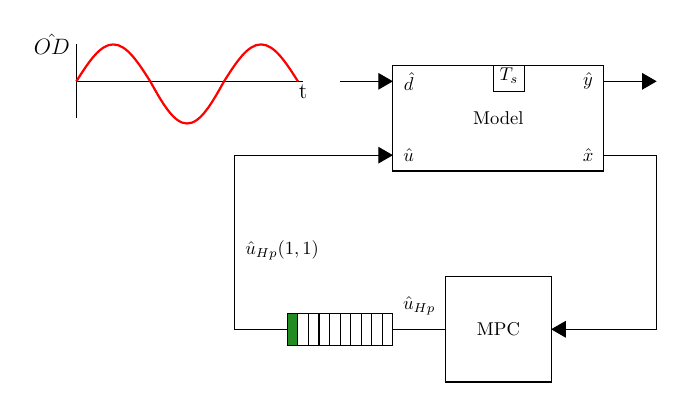
\begin{tikzpicture} [scale=0.67,transform shape]

\draw  (10,2) rectangle (6,0);
\node at (8,1) {Model};
\node at (9.7,1.7) {$\hat{y}$};
\node at (9.7, 0.3) {$\hat{x}$};
\node at (6.3, 1.7) {$\hat{d}$};
\node at (6.3, 0.3) {$\hat{u}$};
\draw[-triangle 60] (10, 1.7) -- (11, 1.7);

\draw[-triangle 60] (10, 0.3) -- (11, 0.3) -- (11,-3) -- (9,-3);

\draw  (9,-2) rectangle (7,-4);
\node at (8,-3) {MPC};
\node at (6.5,-2.55) {$\pmb{\hat{u}_{Hp}}$};
\draw  (7,-3) -- (6,-3);
\draw (6,-3.3) rectangle (4,-2.7);
\draw (8.5,2) rectangle (7.9,1.5);
\node at (8.2,1.8) {$T_s$};

\draw  (5.8,-3.3) -- (5.8,-2.7);
\draw  (5.6,-3.3) -- (5.6,-2.7);
\draw  (5.4,-3.3) -- (5.4,-2.7);
\draw  (5.2,-3.3) -- (5.2,-2.7);
\draw  (5.0,-3.3) -- (5.0,-2.7);
\draw  (4.8,-3.3) -- (4.8,-2.7);
\draw  (4.6,-3.3) -- (4.6,-2.7);
\draw  (4.4,-3.3) -- (4.4,-2.7);
\draw  (4.2,-3.3) -- (4.2,-2.7);
\fill[ForestGreen] (4.18,-3.29) rectangle(4.01,-2.71);
\draw[-triangle 60] (4, -3) -- (3, -3) -- (3,0.3) -- (6,0.3);
\node at (3.9,-1.5) {$\pmb{\hat{u}_{Hp}}(1,1)$};
\draw[-triangle 60] (5,1.7)--(6,1.7);

 
    \draw (0,1.7) -- (4.3,1.7);
    \node [font=\large] at (4.3,1.5) {t};
    \draw (0,2.4)node[left,font=\large] {$\hat{OD}$} -- (0,1.0);
    % \draw (0.2,-1)node[left,font=\tiny] {$y=-1$} -- (11.8,-1); 
    % \foreach \x in {0,0.5,...,12}{
    % \draw (\x,-0.2)node [below,font=\tiny,] {\x} -- (\x,0.2) ;
    % }
    \draw[ thick, red] (0,1.7) sin (0.7,2.4);    %% the real business in this line
    \draw[ thick, red] (0.7,2.4) cos (1.4,1.7);    %% the real business in this line
    \draw[ thick, red] (1.4,1.7) sin (2.1,0.9);    %% the real business in this line
    \draw[ thick, red] (2.1,0.9) cos (2.8,1.7);    %% the real business in this line
    \draw[ thick, red] (2.8,1.7)  sin (3.5,2.4);    %% the real business in this line
    \draw[ thick, red] (3.5,2.4) cos (4.2,1.7);    %% the real business in this line
    % \draw[ultra thick, red] (9,0) sin (10,-1);    %% the real business in this line
    % \draw[ultra thick, blue] (10,-1) cos (11,0);    %% the real business in this line

\end{tikzpicture}%


 
\end{figure}

\end{frame}


\subsection{Implementation results}

\begin{frame}{Implementation results}{For one iteration}

\begin{itemize}
	 	\item<1-> Softened constraints on $\hat{\pmb{\underline{u}}}_{Hp}$
	 	\end{itemize}

\begin{figure}[H]
   \centering
    % This file was created by matlab2tikz.
%
%The latest updates can be retrieved from
%  http://www.mathworks.com/matlabcentral/fileexchange/22022-matlab2tikz-matlab2tikz
%where you can also make suggestions and rate matlab2tikz.
%
\definecolor{mycolor1}{rgb}{0.00000,0.44700,0.74100}%
%
\begin{tikzpicture}

\begin{axis}[%
width=3.028in,
height=0.55in,at={(1.011in,4.137in)},
scale only axis,
xmin=0,
xmax=23,
ymin=-1,
ymax=1,
ylabel={$\hat{P_1}[bar]$},
%xmajorgrids,
%ymajorgrids,
axis background/.style={fill=white},
title style={font=\bfseries},
%title={$\text{u}_{\text{hp1}}\text{[k=0]}$}
]
\addplot[const plot,color=mycolor1,solid,forget plot,very thick] plot table[row sep=crcr] {%
0	-0.433446931217239\\
1	-0.669999999998947\\
2	-0.669999999997713\\
3	-0.104236955958482\\
4	0.749999999997401\\
5	0.749999999998619\\
6	0.727077455814283\\
7	-0.669999999999055\\
8	-0.66999999999925\\
9	-0.395725243988171\\
10	0.749999999988271\\
11	0.749999999998319\\
12	0.717572940373614\\
13	-0.669999999998221\\
14	-0.669999999999149\\
15	-0.409583761852645\\
16	0.548034702463677\\
17	0.749999999998184\\
18	0.74999999999883\\
19	-0.576396407197271\\
20	-0.669999999998877\\
21	-0.425048538821507\\
22	-0.0640667111129486\\
};
\addplot[const plot,color=red,dotted,very thick] plot table[row sep=crcr] {%
0	0.75\\
24	0.75\\
};

\addplot[const plot,color=red,dotted,very thick] plot table[row sep=crcr] {%
0	-0.67\\
24	-0.67\\
};

\end{axis}
\end{tikzpicture}


\begin{tikzpicture}

\begin{axis}[%
width=3.028in,
height=0.55in,
at={(1.011in,2.39in)},
scale only axis,
xmin=0,
xmax=23,
ymin=-1,
ymax=1,
%xmajorgrids,
%ymajorgrids,
ylabel={$\hat{P_2}[bar]$},
axis background/.style={fill=white},
title style={font=\bfseries},
%title={$\text{u}_{\text{hp2}}\text{[k=0]}$}
]
\addplot[const plot,color=mycolor1,solid,forget plot,very thick] plot table[row sep=crcr] {%
0	-0.649999999999008\\
1	-0.649999999999539\\
2	-0.649999999999527\\
3	-0.64999999999887\\
4	-0.649999999994262\\
5	0.0667700518106753\\
6	-0.649999999998485\\
7	-0.649999999999511\\
8	-0.649999999999588\\
9	-0.649999999999157\\
10	-0.649999999997306\\
11	0.0160826405819198\\
12	-0.649999999996155\\
13	-0.64999999999941\\
14	-0.64999999999958\\
15	-0.649999999999219\\
16	-0.649999999998156\\
17	0.189015571020597\\
18	-0.649999999956971\\
19	-0.649999999999335\\
20	-0.649999999999555\\
21	-0.649999999999218\\
22	-0.649999999998207\\
};
\addplot[const plot,color=red,dotted,very thick] plot table[row sep=crcr] {%
0	0.75\\
24	0.75\\
};

\addplot[const plot,color=red,dotted,very thick] plot table[row sep=crcr] {%
0	-0.67\\
24	-0.67\\
};
\end{axis}
\end{tikzpicture}

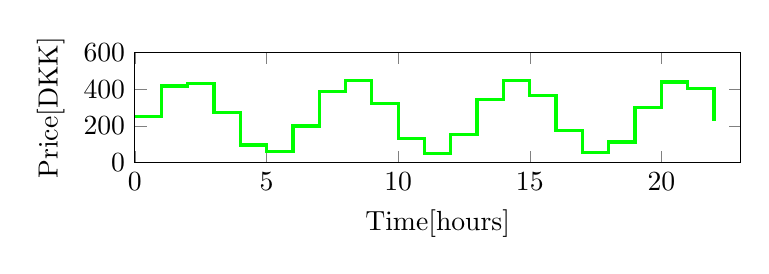
\begin{tikzpicture}

\begin{axis}[%
width=3.028in,
height=0.55in,
at={(1.011in,0.642in)},
scale only axis,
xmin=0,
xmax=23,
xlabel={Time[hours]},
ymin=0,
ymax=600,
%xmajorgrids,
%ymajorgrids,
ylabel={Price[DKK]},
axis background/.style={fill=white},
title style={font=\bfseries},
]
\addplot[const plot,color=green,solid,forget plot,very thick] plot table[row sep=crcr] {%
0	250\\
1	418.857649358291\\
2	430.978019589665\\
3	275.110723996831\\
4	95.9351176989303\\
5	59.7658279797972\\
6	200.175962602534\\
7	386.833833626164\\
8	446.479615730073\\
9	323.748819156816\\
10	132.562792409559\\
11	50.3844917318038\\
12	153.493572208496\\
13	346.181981592006\\
14	449.592219965457\\
15	367.736693884804\\
16	176.595452155304\\
17	53.5898806097876\\
18	112.896379753435\\
19	299.465389524004\\
20	440.119567515206\\
21	404.300699515516\\
22	225.256624358491\\
};
\end{axis}
\end{tikzpicture}%
\end{figure}

\end{frame}


\section{Discussion}
\begin{frame}{Discussion}{}

\begin{itemize}
	\item<1-> Possible improvements and error fixing
	\begin{itemize}
	 \item<1-> Long measurements, ensuring initial steady state condition
	 \item<1-> Correcting the implementation
	 \item<1-> Different softened constraint configurations

	\end{itemize}
\end{itemize}

\begin{itemize}
\item<2-> Considerations for future work
	 \begin{itemize}
	 \item<2-> Using the end-user pressure measurements
	 \item<2-> Robust MPC
	 \item<2-> Non-linear model fixing

		\begin{itemize}
	 	\item<3-> Online linearization
	 	\item<3-> Operating points are constantly varied
	 	\item<3-> Precision is more reliable
	 	\end{itemize}

	 \end{itemize}
\end{itemize}

\end{frame}

%%%%%%%%%%%%%%%%
\section{Discussion}
%%%%%%%%%%%% MID WAY AGENDA %%%%%%%%%%%%%%
 %\begin{frame}<beamer>
 %\frametitle{Nicolaj Vinkel Christensen}
 %\tableofcontents[currentsection]
 %\end{frame}


\begin{frame}{Discussion}{}

\begin{itemize}
	\item<1->The next step
	\begin{itemize}
	 \item<1-> Solving implementation problems  
	 \item<1-> Comparing the results with the real system
	\end{itemize}
\end{itemize}

\begin{itemize}
\item<2-> Future research
	 \begin{itemize}
	 \item<2-> Using a nonlinear model for parameter estimation 
	 \item<2-> Adaptive control
	 \end{itemize}
\end{itemize}

\end{frame}


\section{Conclusion}


\begin{frame}{Conclusion}{}


% \begin{itemize}
% \item<1-> Modelling 
% \begin{itemize}
% \item<1->  A model describing components
% \item<1->  Graph representation of the network  
% \item<1->  Nonlinear parameter identification
% \item<1->  Linearization of the model  
% \item<1->  
% \item<1->  
% \end{itemize}
\begin{itemize}
\item<1-> Hydraulic model 
\begin{itemize}
\item Graph representation
\end{itemize}

\item<1-> Parameter estimation 
\begin{itemize}
\item Nonlinear estimation
\item Linear estimation
\end{itemize}

\item<1-> Control problem
\begin{itemize}
\item Model predictive controller is derived
\end{itemize}

\item<1-> Control implementation
\end{itemize}

\end{frame}





\begin{frame}{Laboratory}{}
\centering{Please follow us to the laboratory}
\end{frame}

\end{document}
